
\documentclass[gmd,noline]{copernicus}

\begin{document}



\title{Addressing numerical challenges in introducing a reactive transport code into a land surface model: a biogeochemical modeling proof-of-concept with CLM--PFLOTRAN 1.0}


\Author[1]{Guoping}{Tang}
\Author[1]{Fengming}{Yuan}
\Author[1,2]{Gautam}{Bisht}
\Author[3,4]{Glenn~E.}{Hammond}
\Author[5]{Peter~C.}{Lichtner}
\Author[1]{Jitendra}{ Kumar}
\Author[6]{Richard~T.}{Mills}
\Author[1,7]{Xiaofeng}{Xu}
\Author[2,8]{Ben}{Andre}
\Author[1]{Forrest~M.}{Hoffman}
\Author[1]{Scott~L.}{Painter}
\Author[1]{Peter~E.}{Thornton}

\affil[1]{Oak Ridge National Laboratory, Oak Ridge, Tennessee, USA}
\affil[2]{Lawrence Berkeley National Laboratory, Berkeley, California, USA}
\affil[3]{Pacific Northwest National Laboratory, Richland, Washington, USA}
\affil[4]{Sandia National Laboratories, Albuquerque, New Mexico, USA}
\affil[5]{OFM Research--Southwest, Santa Fe, New Mexico, USA}
\affil[6]{Intel Corporation, Hillsboro, Oregon, USA}
\affil[7]{San Diego State University, San Diego, California, USA}
\affil[8]{National Center for Atmospheric Research, Boulder, Colorado, USA}



\runningtitle{CLM--PFLOTRAN biogeochemistry}

\runningauthor{G.~Tang et~al.}

\correspondence{P.~E.~Thornton (thorntonpe@ornl.gov) and S. L. Painter (paintersl@ornl.gov)}


\received{18 November 2015}
\pubdiscuss{17 December 2015}
\revised{13 February 2016}
\accepted{17 February 2016}
\published{}

\firstpage{1}

\maketitle


\begin{abstract}
\blackbox[CE]{Note that the abbreviation CLM (Community Land Model) is written as CLMs in the plural form, i.e. Community Land Models.
 There is no need to make it consistent throughout the text. Please check that the singular and plural forms are used correctly.} We explore coupling to a~configurable subsurface reactive transport
      code as a~flexible and extensible approach to biogeochemistry in land
      surface models.
      A~reaction network with
      the Community Land Model carbon--nitrogen (CLM-CN) decomposition, nitrification, denitrification, and plant
      uptake is used as an example. We implement the reactions in the
      open-source PFLOTRAN (massively parallel subsurface flow and reactive transport) code and couple it with the CLM. To make the
      rate formulae designed for use in explicit time stepping in CLMs
      compatible with the implicit time stepping used in PFLOTRAN, the Monod
      substrate rate-limiting function with a~residual concentration is used
      to represent the limitation of nitrogen availability on plant uptake
      and immobilization.
      We demonstrate that CLM--PFLOTRAN predictions (without invoking PFLOTRAN
      transport) are consistent with CLM4.5 for Arctic, temperate, and tropical
      sites.


      Switching from explicit to implicit method increases rigor but introduces
      numerical challenges.
      Care needs to be taken to use scaling, clipping,
      or log transformation to avoid negative concentrations during the
      Newton iterations.
      With a~tight relative update tolerance (STOL) to avoid
      false convergence, an accurate solution can be achieved with about
      50\,{\%} more computing time than CLM in point mode site simulations
      using either the scaling or clipping methods. The log transformation
      method takes 60--100\,{\%} more computing time than CLM. The
      computing time increases slightly for clipping and scaling; it
      increases substantially for log transformation for half saturation
      decrease from $10^{-3}$ to $10^{-9}$\,\unit{mol\,m^{-3}}, which
      normally results in decreasing nitrogen concentrations. The frequent
      occurrence of very low concentrations (e.g.  below nanomolar) can
      increase the computing time for clipping or scaling by about 20\,{\%},
      double for log transformation.
      Overall, the log transformation method is accurate and robust, and the
      clipping and scaling methods are efficient. When the
      reaction network is highly nonlinear or the half saturation or residual
      concentration is very low, the allowable time-step cuts may
      need to be increased for robustness for the log transformation method, or
      STOL may need to be tightened for the clipping and
      scaling methods to avoid false convergence.


      As some biogeochemical processes
      (e.g., methane and nitrous oxide reactions) involve
      very low half saturation and thresholds, this work
      provides insights for addressing nonphysical negativity issues and
      facilitates the representation of a~mechanistic biogeochemical
      description in Earth system models to reduce climate prediction
      uncertainty.
\end{abstract}


\introduction

      Land surface (terrestrial ecosystem) models (LSMs) calculate the
      fluxes of energy, water, and greenhouse gases across the
      land--atmosphere interface for the atmospheric general circulation
      models for climate simulation and weather forecasting
      \citep{Sellers1997}. Evolving from the first generation ``bucket'',
      second generation ``biophysical'', and third generation
      ``physiological'' models \citep{Seneviratne2010}, current LSMs such as
      the Community Land Model (CLM) implement comprehensive thermal,
      hydrological, and biogeochemical processes \citep{Oleson2013}. The
      importance of accurate representation of soil biogeochemistry in LSMs
      is suggested by the confirmation that the increase of carbon dioxide
      (\chem{CO_2}), methane (\chem{CH_4}), and nitrous oxide (\chem{N_2O})
      in the atmosphere since preindustrial time is the main driving cause
      of climate change, and interdependent water, carbon and nitrogen
      cycles in terrestrial ecosystems are very sensitive to climate changes
      \citep{IPCC2013}. In addition to $\sim 250$ soil biogeochemical models
      developed in the past $\sim 80$~years \citep{Manzoni2009},
      increasingly mechanistic models continue to be developed to increase
      the fidelity of process representation for improving climate
      prediction \citep[e.g.,][]{Riley2014}.

      As LSMs usually hardcode the soil biogeochemistry reaction network
      (pools/species, reactions, rate formulae), substantial effort is often
      required to modify the source code for testing alternative models and
      incorporating new process understanding. \citet{Fang2013} demonstrated
      the use of a~reaction-based approach to facilitate implementation of
      the Community Land Model carbon--nitrogen (CLM-CN) and CENTURY models and incorporation of the phosphorus
      cycle.  \citet{Tang2013b} solved the advection diffusion equation in
      CLM using operator splitting. In contrast, TOUGH-REACT, a~reactive
      transport modeling (RTM) code, was used to develop multiphase
      mechanistic carbon and nitrogen models with many speciation and
      microbial reactions \citep{Maggi2008,Gu2010,Riley2014}, but it has not
      been coupled to an LSM. PHREEQC was coupled with DayCent to describe
      soil and stream water equilibrium chemistry
      \citep{Hartman2007}. Coupling a~RTM code with CLM will facilitate
      testing of increasingly mechanistic biogeochemical models in LSMs.

      An essential aspect of LSMs is to simulate competition for nutrients
      (e.g., mineral nitrogen, phosphorus) among plants and microbes. In
      CLMs, plant and immobilization nitrogen demands are calculated
      independent of soil mineral nitrogen. The limitation of nitrogen
      availability on plant uptake and immobilization is simulated by
      a~demand-based competition: demands are downregulated by soil nitrogen
      concentration \citep{Oleson2013,Thornton2005}.  This avoids negative
      concentrations and does not introduce mass balance errors
      \citep{Tang2015} as CLM uses explicit time stepping.
\hack{\newpage}
      RTMs often account for limitation of reactant availability on reaction
      rates for each individual reaction to allow mechanistic
      representations and flexibility in adding reactions. For maximum
      robustness, some RTM codes support the use of fully implicit time
      stepping, usually employing a~variant of the Newton--Raphson
      method. Negative concentration can be introduced during
      Newton--Raphson iterations, which is not physical and can cause
      numerical instability and errors \citep{Shampine2005}. In our work
      with CLMs, this is expected to worsen when we implement microbial
      reactions for methane and nitrous oxide consumption and production as
      the threshold, and half saturation are at or below nanomolar
      ($10^{-9}$\,\unit{M}) level \citep{Conrad1996}. The redox potential
      (Eh)
      needs to be decreased to $-0.35$\,\unit{V} (oxygen concentration
      $<10^{-22}$\,\unit{M}; \citealp{Hungate1975}) for methanogens to grow
      \citep{Jarrell1985}.

      Three methods are used to avoid negative concentration in RTM
      codes. One is to use the logarithm concentration as the primary
      variable \citep{Bethke2007,Hammond2003,Parkhurst1999}. The other two
      either scale back the update vector \citep{Bethke2007,Hammond2003} or
      clip the concentrations for the species that are going negative
      \citep{Yeh2004,White2005,Xu2014} in each iteration. Except that log
      transformation is more computationally demanding \citep{Hammond2003},
      how these methods for enforcing non-negativity affect computational
      accuracy and efficiency is rarely discussed.

      As LSMs need to run under various conditions at the global scale for
      simulation duration of centuries, it is necessary to resolve accuracy
      and efficiency issues to use RTM codes for LSMs. The objective of this
      work is to explore some of the implementation issues associated with
      using RTM codes in LSMs, with the ultimate goal being accurate,
      efficient, robust, and configurable representations of subsurface
      biogeochemical reactions in CLM. To this end, we develop an
      alternative implementation of an existing CLM biogeochemical reaction
      network using PFLOTRAN (massively parallel subsurface flow and reactive transport) \citep{Lichtner2015,Hammond2014}; couple that
      model to CLM (we refer to the coupled model as CLM--PFLOTRAN); test the
      implementation at Arctic, temperate, and tropical sites; and examine
      the implication of using scaling, clipping, and log transformation for
      avoiding negative concentrations.  Although we focus on a~number of
      carbon--nitrogen reactions implemented in PFLOTRAN and CLM, the
      critical numerical issue of avoiding negative concentrations has
      broader relevance as biogeochemical representations in LSMs become
      more mechanistic.



\section{Methods}%s2

      Among the many reactions in LSMs are the soil biogeochemical reactions
      for carbon and nitrogen cycles, in particular the organic matter
      decomposition, nitrification, denitrification,    plant nitrogen uptake,
      and methane production and oxidation.  The kinetics are usually
      described by a~first-order rate modified by response functions for
      environmental variables (temperature, moisture, pH, etc.)
      \citep{Bonan2012,Boyer2006,Schmidt2011}.  In this work, we use
      a~network of the CLM-CN decomposition
      \citep{Bonan2012,Oleson2013,Thornton2005}, nitrification,
      denitrification \citep{Dickinson2002,Parton2001,Parton1996}, and plant
      nitrogen uptake reactions (Fig.~\ref{fig:conceptualmodel}) as an
      example. The reactions and rate formulae are detailed in
      Appendix~\ref{sec:clmbgc}.


%f1
\begin{figure*}[t]
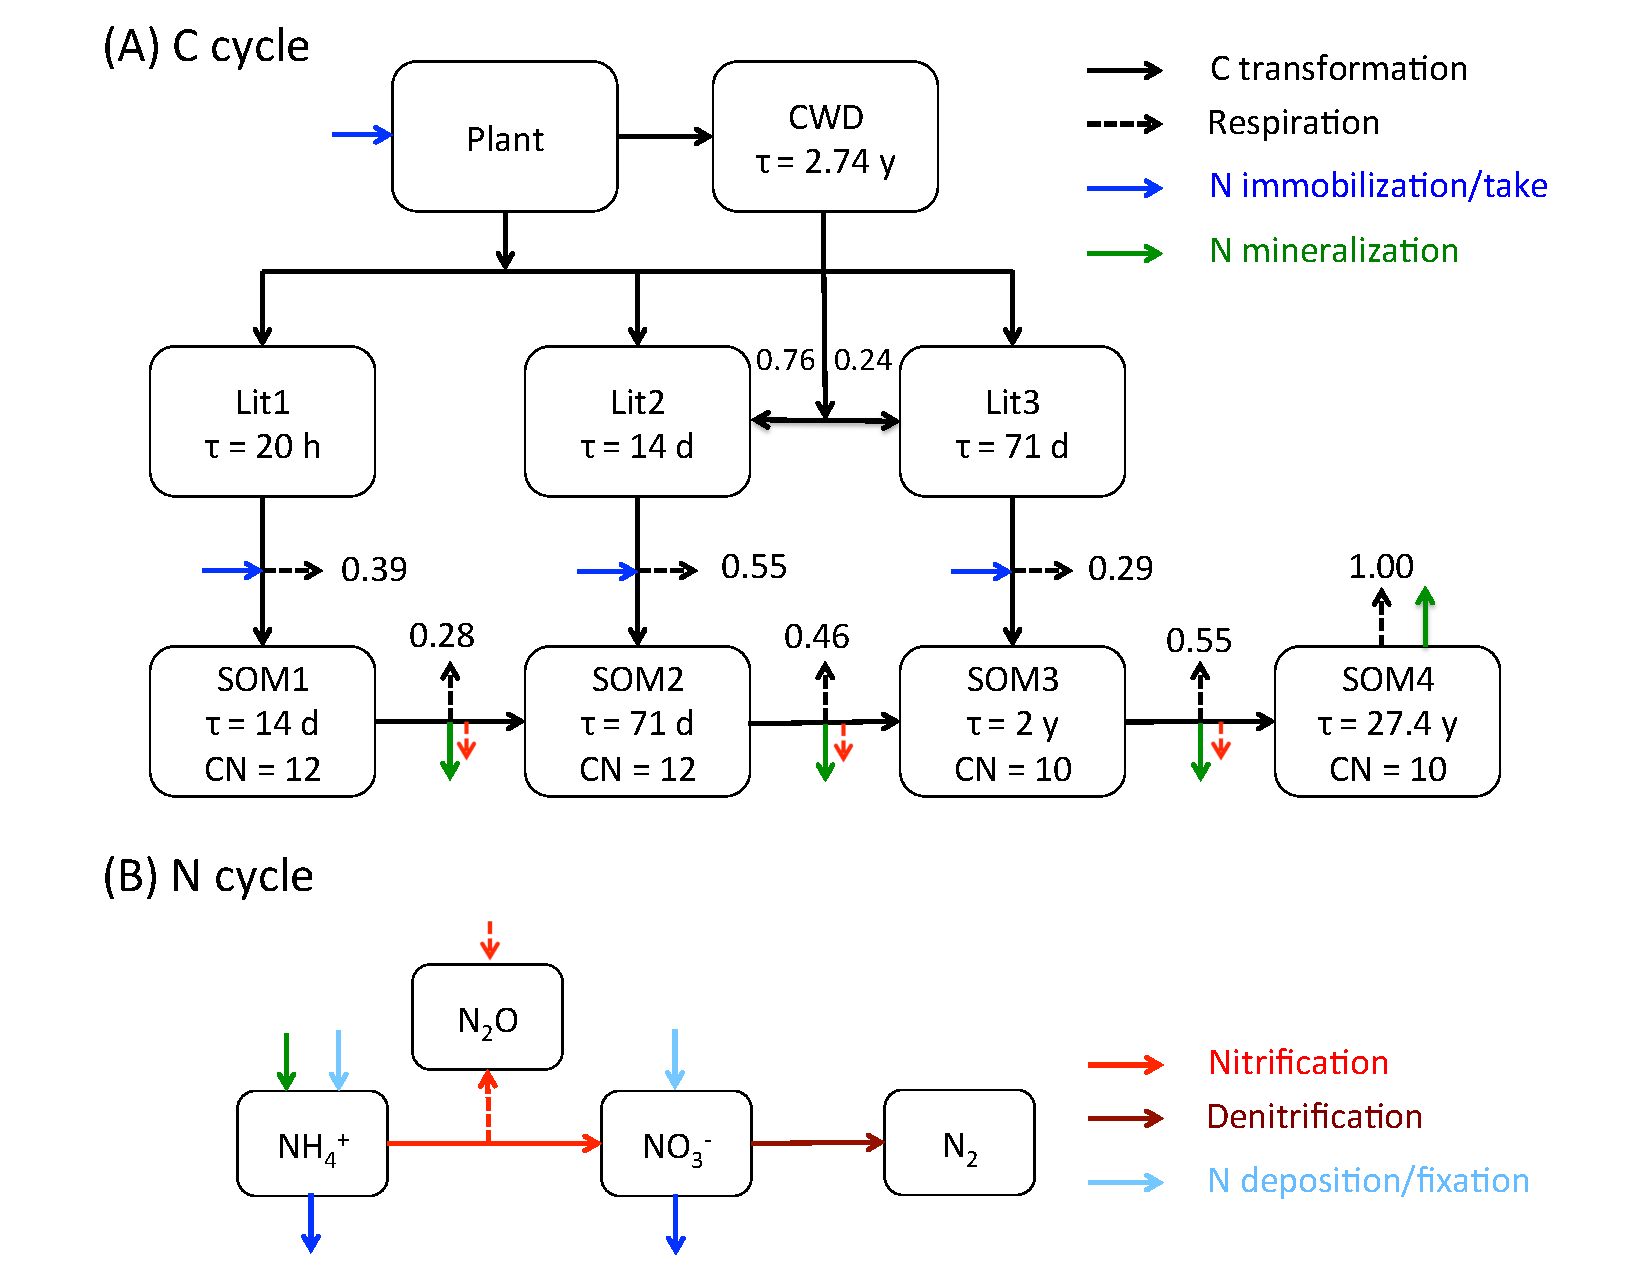
\includegraphics[width=110mm]{gmd-2015-254-f01.pdf}
\caption{The reaction network for the carbon \textbf{(a)}~and nitrogen
\textbf{(b)}~cycles implemented in this work. The carbon cycle is modified
from \citet{Thornton2005} and \citet{Bonan2012}. $\tau$ is the turnover time,
and CN is the CN ratio in g\,C over g\,N.} \label{fig:conceptualmodel}
\end{figure*}




\subsection{CLM--PFLOTRAN biogeochemistry coupling}%s2.1

      In CLM--PFLOTRAN, CLM can instruct PFLOTRAN to solve the partial
      differential equations for energy (including freezing and thawing),
      water flow, and reaction and transport in the surface and
      subsurface. This work focuses on the PFLOTRAN biogeochemistry, with the
      CLM solving the energy and water flow equations and handling the
      solute transport (mixing, advection, diffusion, and leaching).
Here, we focus on how reactions are implemented and thus only use PFLOTRAN in
batch mode (i.e. without transport). However, PFLOTRAN's advection and
diffusion capabilities are operational in the CLM--PFLOTRAN coupling described
here. In each
      CLM time step, the CLM provides production rates for \chem{Lit1C},
      \chem{Lit1N}, \chem{Lit2C}, \chem{Lit2N}, \chem{Lit3C}, \chem{Lit3N}
      for litter fall; \chem{CWDC} and \chem{CWDN} for coarse woody debris
      production, nitrogen deposition and fixation, and plant nitrogen
      demand; and specifies liquid water content, matrix potential, and
      temperature for PFLOTRAN. PFLOTRAN solves ordinary differential
      equations for the kinetic reactions and mass action equations for
      equilibrium reactions and provides the final concentrations back to
      CLM.

      The reactions and rates are implemented using the ``reaction sandbox''
      concept in PFLOTRAN \citep{Lichtner2015}. For each reaction, we
      specify a~rate and a~derivative of the rate with respect to any
      components in the rate formula, given concentrations, temperature,
      moisture content, and other environmental variables (see
      reaction\_sandbox\_example.F90 in pflotran-dev source code for
      details). PFLOTRAN accumulates these rates and derivatives into
      a~residual vector and a~Jacobian matrix, and the global equation is
      discretized in time using the backward Euler method; the resulting
      system of algebraic equations is solved using the Newton--Raphson
      method (Appendix~\ref{sec:newton}).  A~Krylov subspace method is
      usually employed to solve the Jacobian systems arising during the
      Newton--Raphson iterations, but, as the problems are relatively small
      in this study, we solve them directly via LU (lower upper)
      factorization.

      Unlike the explicit time stepping in CLM, in which only reaction rates
      need to be calculated, implicit time stepping requires evaluating
      derivatives.  While PFLOTRAN provides an option to calculate
      derivatives numerically via finite-differencing, we use analytical
      expressions for efficiency and accuracy.

      Many reactions can be specified in an input file, providing
      flexibility in adding various reactions with user-defined rate
      formulae. As typical rate formulae consist of first-order, Monod, and
      inhibition terms, a~general rate formula with a~flexible number of
      terms and typical moisture, temperature, and pH response functions is
      coded in PFLOTRAN. Most of the biogeochemical reactions can be
      specified in an input file, with a~flexible number of reactions,
      species, rate terms, and various response functions without source
      code modification.  Code modification is necessary only when different
      rate formulae or response functions are introduced. In contrast, the
        pools and reactions are traditionally hardcoded in
      CLM. Consequently, any change of the pools, reactions, or rate formula
      may require source code modification. Therefore, the more general
      approach used by PFLOTRAN facilitates implementation of increasingly
      mechanistic reactions and tests of various representations with less
      code modification.


\subsection{Mechanistic representation of rate-limiting processes}%s2.2

      To use RTMs in LSMs, we need to make reaction networks designed for
      use in explicit time-stepping LSMs compatible with implicit time-stepping RTMs. The limitation of reactant availability on reaction
      rate is well represented by the first-order rate
      (Eqs.~\ref{eq:decomprate}, \ref{eq:nitr2no3}, \ref{eq:nitr2n2oexess},
      and~\ref{eq:deni}): the rate decreases to zero as the concentration
      decreases to zero. A~residual concentration \chem{[CN_u]_r} is often
      added to represent a~threshold below which a~reaction stops, for
      example, to the decomposition rate (Eq.~\ref{eq:decomprate}) as
\begin{align}
 &
\frac{\mathrm{d} \chem{[CN_u]}}{\mathrm{d} t} =
-k_{d} f_{T} f_{w} (\chem{[CN_u]} - \chem{[CN_u]_r}).
\label{eq:decomprateresidual}
\end{align}%e1
      Here \chem{CN_u} is the upstream pool with 1\,:\,u as the CN ratio in
      mole; [\,] denotes concentration; and $k_{d}$, $f_{T}$, and
      $f_{w}$ are the rate coefficient, and temperature and moisture response
      functions, respectively. When \chem{CN_u} goes below
      $\chem{[CN_u]_r}$ in an iteration,
      Eq.~(\ref{eq:decomprateresidual}) implies a~hypothetical reverse
      reaction to bring it back to \chem{[CN_u]_r}. The residual
      concentration can be set to zero to nullify the effect.

      For the litter decomposition reactions (Appendix Reactions~\ref{rxn:lit1}--\ref{rxn:lit3}) that immobilize \chem{N},
      the nitrification Reaction~(\ref{rxn:nitr2n2o}) associated with
      decomposition to produce nitrous oxide, and the plant nitrogen uptake
      Reactions~(\ref{rxn:plantatake}) and~(\ref{rxn:plantntake}), the rate
      formulae do not account for the limitation of the reaction rate by
      nitrogen availability.  Mechanistically, a~nitrogen-limiting function
      needs to be added. For example, using the widely used Monod substrate
      limitation function \citep{Fennell1998},
      Eq.~(\ref{eq:decomprateresidual}) becomes\hack{\newpage}
\begin{align}
 &
\hack{\hbox\bgroup\fontsize{9.5}{9.5}\selectfont$\displaystyle}\frac{\mathrm{d}
\chem{[CN_u]}}{\mathrm{d} t} = -k_{d} f_{T} f_{w} (\chem{[CN_u]} -
\chem{[CN_u]_r}) \frac{\chem{[N]}-\chem{[N]_r}}{\chem{[N]}-\chem{[N]_r}
+k_\mathrm{m}},\hack{$\egroup} \label{eq:decompresidualnlimit}
\end{align}%e2
      with half saturation $k_\mathrm{m}$ and a~mineral nitrogen residual
      concentration \chem{[N]_r}. In the case of
      \chem{[N]}--\chem{[N]_r}\,$=$\,$k_\mathrm{m}$, the rate-limiting function is equal to 0.5. For
      \chem{[N]} $\gg k_\mathrm{m}$, Eq.~(\ref{eq:decompresidualnlimit})
      approximates zero order with respect to \chem{[N]}. For $\chem{[N]}\ll
      k_\mathrm{m}$, Eq.~(\ref{eq:decompresidualnlimit}) approximates first
      order with respect to \chem{[N]}. The derivative of the Monod term,
      ${k_\mathrm{m}}{(\chem{[N]}+k_\mathrm{m})^{-2}}$, increases to about
      $k_\mathrm{m}^{-1}$ as the concentration decreases to below
      $k_\mathrm{m}$. This represents a~steep transition when $k_\mathrm{m}$ is
      small. The half saturation is expected to be greater than the residual
      concentration. When both are zero, the rate is not limited by the
      substrate availability.

      To separate mineral nitrogen into ammonium (\chem{NH_4^+}) and nitrate
      (\chem{NO_3^-}), it is necessary to partition the demands between
      ammonium and nitrate for plant uptake and immobilization. If we
      simulate the ammonium limitation on plant uptake with
\begin{align}
 &
R_\mathrm{a} = R_\mathrm{p} \frac{[\chem{NH_4^+}]}{[\chem{NH_4^+}]+k_\mathrm{m}},
\label{eq:plantarate}
\end{align}%e3
      the plant nitrate uptake can be represented by\hack{\newpage}
\begin{align}
 &
R_\mathrm{n} = (R_\mathrm{p} - R_\mathrm{a})
\frac{[\chem{NO_3^-}]}{[\chem{NO_3^-}]+k_\mathrm{m}}\nonumber\\& =
R_\mathrm{p} \frac{k_\mathrm{m}}{[\chem{NH_4^+}]+k_\mathrm{m}}
\frac{[\chem{NO_3^-}]}{[\chem{NO_3^-}]+k_\mathrm{m}}. \label{eq:plantnrate}
\end{align}%e4

      In this equation $R_\mathrm{p}$, $R_\mathrm{a}$, and $R_\mathrm{n}$
      are the plant uptake rates for nitrogen, ammonium
      (Reaction~\ref{rxn:plantatake}), and nitrate
      (Reaction~\ref{rxn:plantntake}). $R_\mathrm{p}$ is calculated in the CLM and input
      to PFLOTRAN as a~constant during each CLM time
      step. Equation~(\ref{eq:plantnrate}) essentially assumes an inhibition
      of ammonium on nitrate uptake, which is consistent with the
      observation that plant nitrate uptake rate remains low until ammonium
      concentrations drop below a~threshold \citep{eltrop1996}.  However,
      the form of the rate expression will differ for different plants
      \citep{Pfautsch2009,Warren2007,Nordin2001,Falkengren1995,Gherardi2013},
      which will require different representations in future developments.

      CLM uses a~demand-based competition approach (Appendix~A,
      Sect.~\ref{sec:demandbasedcompetition}) to represent the limitation of
      available nitrogen on plant uptake and immobilization. It is similar
      to the Monod function except that it introduces a~discontinuity during
      the transition between the zero and first-order rate. Implementation
      of the demand-based competition in a~RTM involves separating the
      supply and consumption rates for each species in each reaction and
      limiting the consumption rates if supply is less than demand after
      contributions from all of the reactions are accumulated. It involves
      not only the rate terms for the residual but also the derivative terms
      for the Jacobian. The complexity increases quickly when more species
      need to be downregulated (e.g., ammonium, nitrate, and organic
      nitrogen) and there are transformation processes among these
      species. It becomes challenging to separate, track, and downregulate
      consumption and production rates for an indefinite number of species,
      and calculation of the Jacobian becomes convoluted. In contrast, use
      of the Monod function with a~residual concentration for individual
      reactions is easier to implement and allows for more flexibility in adding
      reactions.



\subsection{Scaling, clipping, and log transformation for avoiding negative concentration}%s2.3

      Negative components of the concentration update ($\delta
      \vec{c}^{k+1,p+1}$ for iteration $p$ from time-step $k$ to $k+1$ in
      a~Newton--Raphson iteration) can result in negative concentration in
      some entries of $\vec{c}^{k+1,p}$ (Eq.~\ref{eq:update}), which is
      nonphysical. One approach to avoid negative concentration is to scale
      back the update with a~scaling factor ($\lambda$)
      \citep{Bethke2007,Hammond2003} such that
\begin{align}
 &
\vec{c}^{k+1,p+1}=\vec{c}^{k+1,p}+\lambda \delta \vec{c}^{k+1,p+1} > 0,
\label{eq:lambda}
\end{align}%e5
      where
\begin{align}
 &
\lambda = \min_{i=0,m} [1, \alpha {\vec{c}^{k+1,p}(i)}/{\delta \vec{c}^{k+1,p+1} (i)}]
\label{eq:alpha}
\end{align}%e6
      for negative $\delta \vec{c}^{k+1,p+1} (i)$ with $m$ as the number of
      species times the number of numerical grid cells and $\alpha$ as
      a~factor with default value of 0.99. A~second approach, used by RTM
      codes STOMP, HYDROGEOCHEM 5.0, and TOUGH-REACT, is clipping (i.e., for
      any $\delta \vec{c}^{k+1,p+1}(i) \geq \vec{c}^{k+1,p}(i)$, $\delta
      \vec{c}^{k+1,p+1}(i) = \vec{c}^{k+1,p}(i) - \epsilon$ with $\epsilon$ as
      a~small number, e.g., $10^{-20}$). This limits the minimum
      concentration that can be modeled.

      A~third approach, log transformation, also ensures a~positive solution
      \citep{Bethke2007,Hammond2003,Parkhurst1999}. It is widely used in
      geochemical codes for describing highly variable concentrations for
      primary species such as \chem{H^+} or \chem{O_2} that can vary over
      many orders of magnitude as pH or redox state changes without the need
      to use variable switching. Instead of solving Eq.~(\ref{eq:residual})
      for $\vec{c}^{k+1}$ using Eqs.~(\ref{eq:jacobian})--(\ref{eq:update}),
      this method solves for ($\ln\vec{c}^{k+1}$) \citep{Hammond2003} with
\begin{align}
 &
\mathbf{J}_{\ln}(i, j) =
\frac{\partial {f}(i)}{\partial \ln(\vec{c}(j))} = \vec{c}(j) \frac{\partial {f}(i)}{\partial \vec{c}(j)} = \vec{c}(j) \mathbf{J}(i, j),
\label{eq:jacobianlt}\\
&
\delta \ln\vec{c}^{k+1,p+1}= -\mathbf{J}^{-1}_{\ln} {f} (\vec{c}^{k+1,p}),
\label{eq:axblt}
\end{align}%e7 e8
      and
\begin{align}
 &
\vec{c}^{k+1,p+1}=\vec{c}^{k+1,p}\exp [\delta \ln(\vec{c}^{k+1,p+1})].
\label{eq:updatelt}
\end{align}%e9


\section{Tests, results, and discussions}%s3

      The Newton--Raphson method and scaling, clipping, and log
      transformation are widely used and extensively tested for RTMs, but
      not for coupled LSM--RTM applications. The CLM describes biogeochemical
      dynamics within daily cycles for simulation durations of hundreds of
      years; the nitrogen concentration can be very low (\unit{mM} to
      \unit{nM}) while the carbon concentrations can be very high (e.g.,
      thousands \unit{mol\,m^{-3}} carbon in an organic layer); the
      concentrations and dynamics can vary dramatically in different
      locations around the globe. It is not surprising that the complex
      biogeochemical dynamics in a~wide range of temporal and spatial scales
      in CLM poses numerical challenges for the RTM methods. Our simulations
      reveal some numerical issues (errors, divergence, and small time-step
      sizes) that were not widely reported. We identify the issues from
      coupled CLM--PFLOTRAN simulations and reproduce them in simple test
      problems. We examine remedies in the simple test problems and test
      them in the coupled simulations.

      For tests 1--3, we start with plant ammonium uptake to examine the
      numerical solution for Monod function, and then add nitrification and
      denitrification incrementally to assess the implications of adding
      reactions. For test 4, we check the implementation of mineralization
      and immobilization in the decomposition reactions. Third, we compare
      the nitrogen demand partition into ammonium and nitrate between CLM
      and PFLOTRAN. With coupled CLM--PFLOTRAN spin-up simulations for
      Arctic, temperate, and tropical sites, we assess the application of
      scaling, clipping, and log transformation to achieve accurate,
      efficient, and robust simulations. Spreadsheets, PFLOTRAN input
      files, and additional materials are provided as Supplement, and archived
      at \citeauthor{Tang2016}(\citeyear{Tang2016}).

      Our implementation of CLM soil biogeochemistry introduces mainly two
      parameters: half saturation ($k_\mathrm{m}$) and residual
      concentration. A~wide range of $k_\mathrm{m}$ values was reported for
      ammonium, nitrate, and organic nitrogen for microbes and plants. The
      median, mean, and standard deviations range from 10 to 100, 50 to 500, and 10 to 200\,\unit{{\mu}M}, respectively
      \citep{Kuzyakov2013}. Reported residual concentrations are limited --
      likely because of the detection limits of the analytical methods --
      and are considered to be zero \cite[e.g.,][]{Hogh1997}. The detection
      limits are usually at the micromolar level, while up to the nanomolar
      level was reported \citep{Nollet2013}. In Ecosys, the $k_\mathrm{m}$ is
      0.40 and 0.35\,\unit{g\,N\,m^{-3}}, and the residual concentration is
      0.0125 and 0.03\,\unit{g\,N\,m^{-3}} \citep{Grant2013} for ammonium
      and nitrate for microbes, respectively. We start with $k_\mathrm{m}=10^{-6}$\,\unit{M} or
      \unit{mol\,m^{-3}}, and residual
      concentration\,$=$\,$10^{-15}$\,\unit{M} or \unit{mol\,m^{-3}} for
      plants and microbes. To further investigate the nonphysical solution
      negativity for the current study and for future application for other
      reactants (e.g., \chem{H_2} and \chem{O_2}) where the concentrations
      can be much lower, we examine $k_\mathrm{m}$ from 10$^{-3}$ to $10^{-9}$ in our
      test problems. The $k_\mathrm{m}$ is expected to be different for
      different plants, microbes, and for ammonium and nitrate. We do not
      differentiate them in this work as we focus on numerical issues.



\subsection{Simple tests}%s3.1

\subsubsection{Plant nitrogen uptake, nitrification, and denitrification}%s3.1.1
\label{sec:test1}

      It was observed that plants can decrease nitrogen concentration to
      below the detection limit in hours \citep{Kamer2001}. In CLM, the
      total plant nitrogen demand is calculated based on photosynthesized
      carbon allocated for new growth and the C\,:\,N stoichiometry for new
      growth allocation, and the plant nitrogen demand from the soil
      ($R_\mathrm{p}$) is equal to the total nitrogen demand minus
      retranslocated nitrogen stored in the plants \citep{Oleson2013}. The
      demand is provided as an input to PFLOTRAN. We use the Monod function
to represent the limitation of nitrogen availability on uptake. Once the
plant nitrogen uptake is calculated in PFLOTRAN, it is returned to CLM, which
allocates the uptake among, leaf, live stem, dead stem, etc., and
associated storage pools \citep{Oleson2013}. We
      examine the numerical solutions for the Monod equation at
      first. Incrementally, we add first-order reactions (e.g.,
      nitrification, denitrification, and plant nitrate uptake) to look into
      the numerical issues in increasingly complex reaction networks.

%{\hack{\vspace*{1\baselineskip}}}

%\hack{\noindent}\textit{

\subsubsection*{Plant ammonium uptake (test 1)}

      We consider the plant ammonium uptake Reaction~(\ref{rxn:plantatake})
      with a~rate $R_\mathrm{a}$
\begin{align}
 &
\frac{\mathrm{d} [\chem{NH_4^+}]}{\mathrm{d} t} =
- R_\mathrm{a} \frac{[\chem{NH_4^+}]}{[\chem{NH_4^+}]+k_\mathrm{m}}.
\label{eq:ex1}
\end{align}%e10

      Discretizing it in time using the backward Euler method for a~time-step size $\Delta t$, a~solution is
\begin{align}
 &
[\chem{NH_4^+}]^{k+1} = 0.5 \left[ [\chem{NH_4^+}]^k - k_\mathrm{m} -
R_\mathrm{a} \Delta t \pm \right.\nonumber\\&
\left.\sqrt{\left([\chem{NH_4^+}]^k - k_\mathrm{m} - R_\mathrm{a}\Delta
t\right)^2 + 4 k_\mathrm{m}[\chem{NH_4^+}]^k} \right]. \label{eq:monodsemi}
\end{align}%e11

      Ignoring the negative root, [\chem{NH_4^+}]$^{k+1}\geq 0$. Adding
      a~residual concentration by replacing [\chem{NH_4^+}] with
      $[\chem{NH_4^+}]-\chem{[NH_4^+]_r}$,
      $[\chem{NH_4^+}]\geq\chem{[NH_4^+]_r}$.  Namely, the representation of
      plant ammonium uptake with the Monod function mathematically ensures
      $[\chem{NH_4^+}]^{k+1} \geq \chem{[NH_4^+]_r}$.

      We use a~spreadsheet to examine the Newton--Raphson iteration process
      for solving Eq.~(\ref{eq:ex1}) and the application of clipping,
      scaling, and log transformation (test1.xlsx  in the Supplement). When an overshoot
      gets the concentration closer to the negative than the positive root
      (Eq.~\ref{eq:monodsemi}), the iterations converge to the nonphysical
      negative semianalytical solution (spreadsheet case3).  This can be
      avoided by using clipping, scaling, or log transformation (spreadsheet
      case4, case6, case8).

      Even though clipping avoids convergence to the negative solution, the
      ammonium consumption is clipped, but the \chem{PlantA}  (Reaction AR13) production is
      not clipped (spreadsheet case5), violating the reaction
      stoichiometry. This results in mass balance errors for explicit time
      stepping \citep{Tang2015}. For implicit time stepping, additional
      iterations can resolve this violation to avoid mass balance error.
      However, if a~nonreactive species is added with a~concentration of
      1000\,\unit{mol\,m^{-3}} (e.g., soil organic matter pool 4 SOM4 in
      organic layer), the relative update $\text{snorm}_{\text{rel}}= {\vert\vert
      \delta \vec{c}^{k+1,p} \vert\vert_2} / {\vert\vert \vec{c}^{k+1,p} \vert\vert
      _2}$ decreases to $9.3\times 10^{-9}$ in the iteration (spreadsheet
      case5a). With a~relative update tolerance (STOL; Eq.~\ref{eq:stol}) of
      $10^{-8}$, the iteration would be deemed converged. This false
      convergence may produce mass balance error. Satisfying the relative
      update tolerance criteria does not guarantee that the residual
      equations are satisfied \citep{Lichtner2015}. For this reason, we need
      a~tight STOL to avoid this false convergence so that additional
      iterations can be taken to solve the residual equation accurately.

      In contrast to clipping, scaling applies the same scaling factor to
      limit both ammonium consumption and \chem{PlantA} production following
      the stoichiometry of the reaction~(spreadsheet case6). However, if we
      add a~production reaction that is independent of plant ammonium
      uptake, say nitrate deposition, which can come from CLM as a~constant
      rate in a~time step rather than an internally balanced reaction,
      scaling reduces the plant ammonium uptake to account for the
      availability of ammonium as we intend, but the nitrate deposition rate
      is also reduced by the same scaling factor even though it is not
      limited by the availability of either ammonium or nitrate (spreadsheet
      case7). Like clipping, this unintended consequence can be resolved in
      the subsequent iterations, and a~loose STOL may lead to false
      convergence and mass balance errors.

      Small to zero concentration for ammonium and \chem{PlantA} has no
      impact on the iterations for the clipping or scaling methods in this
      test. In contrast, a~small initial \chem{PlantA} concentration can
      cause challenges for the log transformation method even though
      \chem{PlantA} is only a~product. When it is zero, the Jacobian matrix
      is singular because zero is multiplied to the column corresponding to
      \chem{PlantA} (Eq.~\ref{eq:jacobianlt}). An initial \chem{PlantA}
      concentration of $10^{-9}$ can result in underflow of the exponential
      function (spreadsheet caseA, as a~64-bit real number (``double
      precision''), is precise to 15 significant digits and has a~range of
      $e^{-709}$ to $e^{709}$ in IEEE 754 floating-point representation;
      \citealp{Lemmon2005}).  Clipping the update (say to be between $-$5 and
      5) is needed to prevent numerical overflow or underflow. Like the
      cases with clipping without log transformation, clipping violates
      reaction stoichiometry in the clipping iteration, and this violation
      needs to be resolved in subsequent iterations (spreadsheet caseB).

      This simple test for the Monod function indicates that
      (1)~Newton--Raphson iterations may converge to a~negative
      concentration; (2)~scaling, clipping, and log transformation can be
      used to avoid convergence to negative concentration; (3)~small or zero
      concentration makes the Jacobian matrix stiff or singular when log
      transformation is used, and clipping is needed to guard against
      overflow or underflow of the exponential function; (4)~clipping limits
      the consumption, but not the corresponding production, violating
      reaction stoichiometry in the iteration; (5)~production reactions with
      external sources are inhibited in the iterations when scaling is
      applied, which is unintended; (6)~additional iterations can resolve
      issues in~(4) or~(5); and (7)~loose update tolerance convergence
      criteria may cause false convergence and result in mass balance errors
      for clipping and scaling.

%{\hack{\vspace*{1\baselineskip}}}

%\hack{\noindent}\textit{

\subsubsection*{Plant ammonium uptake and nitrification (test 2)}

      Adding a~nitrification Reaction~(\ref{rxn:nitr2no3}) with
      a~first-order rate to the plant ammonium uptake Reaction
      (\ref{rxn:plantatake}), Eq.~(\ref{eq:ex1}) becomes
\begin{align}
 &
\frac{\mathrm{d} [\chem{NH_4^+}]}{\mathrm{d}t} = - R_\mathrm{a}
\frac{[\chem{NH_4^+}]}{[\chem{NH_4^+}]+k_\mathrm{m}} \nonumber\\&-
k_{\text{nitr}} [\chem{NH_4^+}] = -R_{\text{at}} - R_{\text{nitr}}.
\label{eq:ex2}
\end{align}%e12

      A~semianalytical solution similar to Eq.~(\ref{eq:monodsemi}) can be
      derived for Eq.~(\ref{eq:ex2}). With $J_{\text{at}} = \mathrm{d}
      R_{\text{at}}/\mathrm{d} [\chem{NH_4^+}] =
      R_\mathrm{a}k_\mathrm{m}([\chem{NH_4^+}] + k_\mathrm{m})^{-2}$, and
      $J_{\text{nitr}} = \mathrm{d} R_{\text{nitr}}/\mathrm{d}
      [\chem{NH_4^+}]=k_{\text{nitr}}$, the matrix equation
      Eq.~(\ref{eq:axb}) becomes
\begin{align}
 &
\left[
\begin{matrix}
1/\Delta t + J_{\text{at}} + J_{\text{nitr}} & 0 & 0 \\
-J_{\text{at}} & 1/\Delta t & 0 \\
-J_{\text{nitr}} & 0 & 1/\Delta t \\
\end{matrix}
\right]\nonumber\\& \left(\begin{matrix}
\delta [\chem{NH_4^+}]^{k+1,1} \\
\delta [\chem{PlantA}]^{k+1,1} \\
\delta [\chem{NO_3^-}]^{k+1,1}
\end{matrix}
\right)
=-
\left(\begin{matrix}
R_{\text{at}} + R_{\text{nitr}} \\
-R_{\text{at}} \\
-R_{\text{nitr}}
\end{matrix}
\right),
\label{eq:test2}
\end{align}%e13
      for the first iteration. As $R_{\text{at}} + R_{\text{nitr}} \geq 0$,
      the ammonium update is negative even when the ammonium concentration
      is not very low. The off-diagonal terms for \chem{PlantA} and nitrate
      in the Jacobian matrix bring the negative ammonium update into the
      updates for \chem{PlantA} and nitrate even though there is no reaction
      that consumes them. Specifically,
\begin{align}
 &
\frac{\delta [\chem{PlantA}]^{k+1,1}}{\Delta t} = \frac{\frac{1}{\Delta t} +
J_{\text{nitr}}}{\frac{1}{\Delta t} + J_{\text{at}} +
J_{\text{nitr}}} R_{\text{at}}\nonumber\\& - \frac{J_{\text{at}}}
{\frac{1}{\Delta t} + J_{\text{at}} + J_{\text{nitr}}} R_{\text{nitr}},
\\
& \frac{\delta [\chem{NO_3^-}]^{k+1,1}}{\Delta t} =
-\frac{J_{\text{nitr}}}{\frac{1}{\Delta t} + J_{\text{at}} + J_{\text{nitr}}}
R_{\text{at}} \nonumber\\& + \frac{\frac{1}{\Delta t} + J_{\text{at}}}
{\frac{1}{\Delta t} + J_{\text{at}} + J_{\text{nitr}}} R_{\text{nitr}}.
\end{align}%e14 e15

      Depending on the rates ($R_{\text{at}}$, $R_{\text{nitr}}$),
      derivatives ($J_{\text{at}}$, $J_{\text{nitr}}$), and time-step size
      $\Delta t$, the update can be negative for \chem{PlantA} and nitrate,
      producing a~zero-order ``numerical consumption'', in which the
      limitation of availability is not explicitly represented. This has
      implications for the scaling method.

%f2
\begin{figure*}[t]
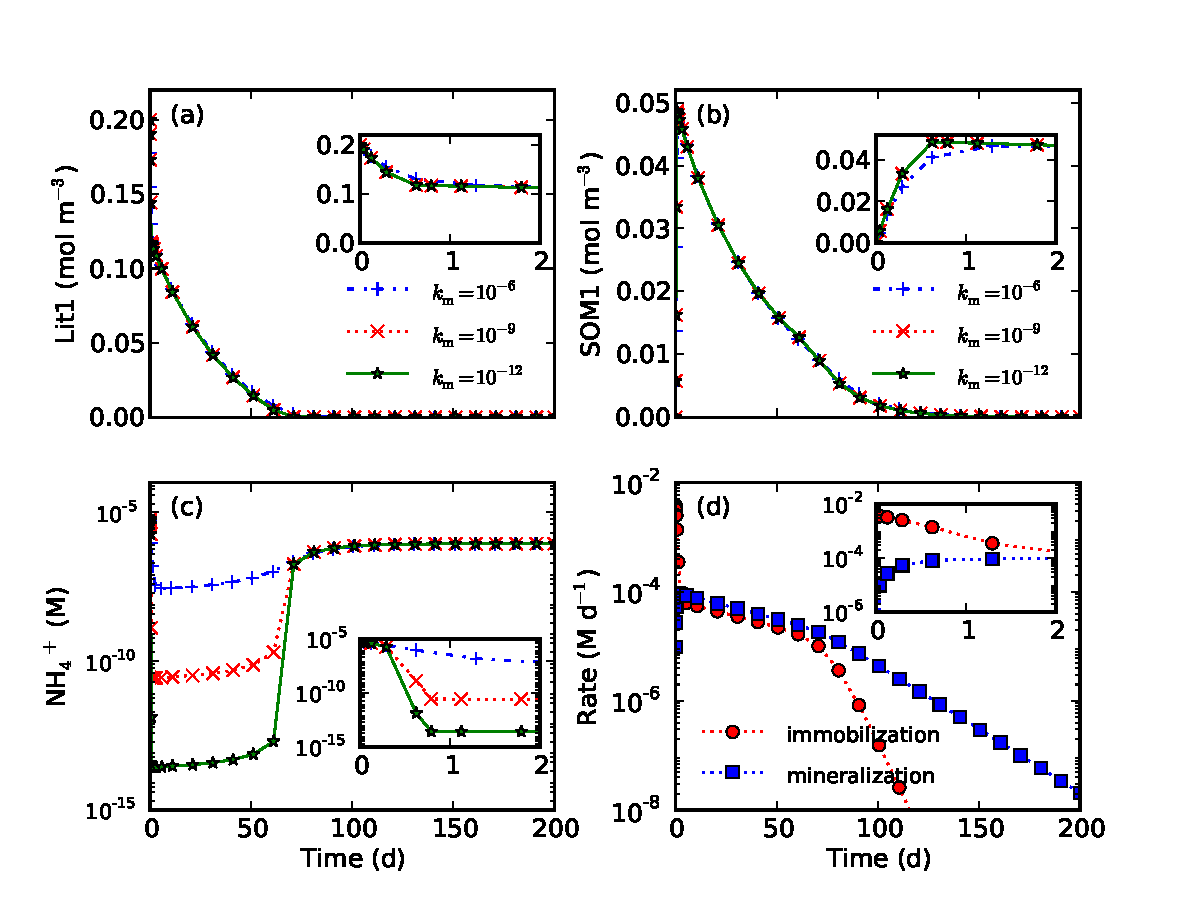
\includegraphics[width=110mm]{gmd-2015-254-f02.pdf}
\caption{Influence of half saturation $k_\mathrm{m}$ on decomposition that
involves both nitrogen immobilization and mineralization. Smaller half
saturation can result in lower nitrogen concentration~\textbf{(c)} but does
not substantially impact the calculated concentrations other than
ammonium~\textbf{(a,\,b)}.} \label{fig:decomp}
\end{figure*}


      The scaling factor ($\lambda$) is a~function of not only the update
      but also the concentration (Eq.~\ref{eq:alpha}). If
      a~negative update is produced for a~zero concentration, the scaling
      factor is zero, decreasing the scaled update to zero. The iteration
      converges without any change to the concentrations, numerically
      stopping all of the reactions in the time step unless STOL is
      negative. We add the denitrification reaction with $R_{\text{nitr}} =
      10^{-6}$\,\unit{s^{-1}} to  test1.xlsx case6 (Supplement) to create  test2.xlsx
      (Supplement)
      to demonstrate that a~small enough initial concentration relative to
      the negative update may numerically inhibit all of the reactions as
      well.  An update of $-6.6 \times 10^{-6}$\,\unit{M} is produced for
      nitrate (spreadsheet scale1). When the initial nitrate concentration
      [\chem{NO_3^-}]$_0$ is not too small, say $10^{-6}$\,\unit{M}, the
      solution converges to the semianalytical solution in six
      iterations. When [\chem{NO_3^-}]$_0$ is decreased to
      10$^{-9}$\,\unit{M}, the relative update $\text{snorm}_{\text{rel}}$
      is $9.2\times 10^{-10}$. If STOL\,$=$\,$10^{-9}$, the solution is
      deemed converged as Eq.~(\ref{eq:stol}) is met, but not to the
      positive semianalytical solution. The ammonium uptake and
      nitrification reactions are numerically ``inhibited'' because the
      small scaling factor and a~high concentration of a~nonreactive species
      decreases the update to below STOL to reach false convergence. If we
      tighten STOL to $10^{-30}$, the iterations continue, with decreasing
      nitrate concentration, $\lambda$, and $\text{snorm}_{\text{rel}}$ by
      2 orders of magnitude ($1-\alpha$ as default $\alpha=0.99$) in each
      iteration, until $\text{snorm}_{\text{rel}}$ reaches $10^{-30}$
      (spreadsheet scale2). Unless STOL is sufficiently small, or MAXIT (the
      maximum number of iterations before stopping the current iterations
      and cutting the time step) is small (Appendix~\ref{sec:newton}), false
      convergence is likely to occur for the scaling method. The impact of
      ``numerical consumption'' on clipping and log transformation is much
      less dramatic than the scaling method as the latter applies the same
      scaling factor to the whole update vector following stoichiometric
      relationships of the reactions to maintain mass balance, and the
      limiting concentration decreases by $(1-\alpha)$ times in each
      iteration, with the possibility of resulting in less than STOL
      relative update in MAXIT iterations.

      In summary, this test problem demonstrates that (1)~a~negative update
      can be produced even for products during a~Newton--Raphson iteration;
      and (2)~when a~negative update is produced for a~very low
      concentration, a~very small scaling factor may numerically inhibit all
      of the reactions due to false convergence even with very tight STOL.


%{\hack{\vspace*{1\baselineskip}}}

%\hack{\noindent}\textit{

\subsubsection*{Plant uptake, nitrification, and denitrification (test~3)}

      The matrix and update equations with plant nitrate uptake and
      denitrification added to test 2 are available in
      Appendix~\ref{sec:eqtest3}. In addition to nitrate and PlantA, PlantN  (Reaction AR14)
      and the denitrification product nitrogen gas may have negative
      updates. In addition to the off-diagonal terms due to the derivative
      of plant uptake with respect to ammonium concentration, the derivative
      of plant uptake with respect to nitrate concentration is added in the
      Jacobian matrix for \chem{PlantN} (Eq.~\ref{eq:complexjacobian}). As
      a~result, a~negative update for both ammonium and nitrate contributes
      to negative \chem{PlantN} update through the two nonzero off-diagonal
      terms.  Therefore, the likelihood for a~negative update to
      \chem{PlantN} is greater than \chem{PlantA} as the former is
      influenced by more rates and derivatives. We add plant nitrate uptake
      and denitrification into test2.xlsx (Supplement) and assess the implications of
      increased reactions and complexity in test3.xlsx (Supplement). In addition to
      nitrate, this introduces a~negative update for nitrogen gas in the
      first iteration (spreadsheet scale1).  As the iterations resolve the
      balance between nitrite production from nitrification, and consumption
      due to plant uptake and denitrification, update to PlantN becomes
      negative and eventually leads to false convergence. The time-step size
      needs to be decreased from 1800 to 15\,\unit{s} to resolve the false
      convergence (spreadsheet scale2). In contrast, the added reactions
      have less impact on the clipping and log transformation methods.


\subsubsection{Nitrogen immobilization and mineralization during decomposition (test~4)}%s3.1.2



      We examine another part of the reaction network: decomposition,
      nitrogen immobilization, and mineralization
      (Fig.~\ref{fig:conceptualmodel}). We consider a~case of decomposing
      0.2\,\unit{M} \chem{Lit1C}\,$+$\,0.005\,\unit{M} \chem{Lit1N} to
      produce \chem{SOM1} with initial 4\,\unit{{\mu}\,M} ammonium using the
      reactions~(\ref{rxn:som1}) and~(\ref{rxn:lit1}) in the CLM-CN reaction
      network (Fig.~\ref{fig:conceptualmodel}). We use PFLOTRAN with
      a~water-saturated grid cell with porosity of 0.25. At the beginning,
      Lit1 decreases and SOM1 increases sharply because the rate coefficient
      for Lit1 is 16 times that for SOM1 (Fig.~\ref{fig:decomp}a~and~b). As
      ammonium concentration decreases by orders of magnitude because of the
      faster immobilization than mineralization rate
      (Fig.~\ref{fig:decomp}c~and~d), Lit1 decomposition rate slows down to
      the level such that the immobilization rate is less than the
      mineralization rate. Namely, SOM1 decomposition controls Lit1
      decomposition through limitation of mineralization on
      immobilization. As the immobilization rate decreases with decreasing
      Lit1, ammonium concentration rebounds after Lit1 is depleted. For
      $k_\mathrm{m}$ values of 10$^{-6}$, 10$^{-9}$, and 10$^{-12}$\,M,
      \chem{Lit1} and \chem{SOM1} dynamics are similar except for slight
      differences in the early transit periods, but the ammonium values are
      decreased to $\sim 1 0^{-8}$, 10$^{-11}$, and 10$^{-14}$\,M,
      respectively. Smaller $k_\mathrm{m}$ values result in lower ammonium
      concentrations, which have implications for the clipping, scaling, and
      log transformation methods as discussed in tests~1--3.


%f3
\begin{figure*}[t]
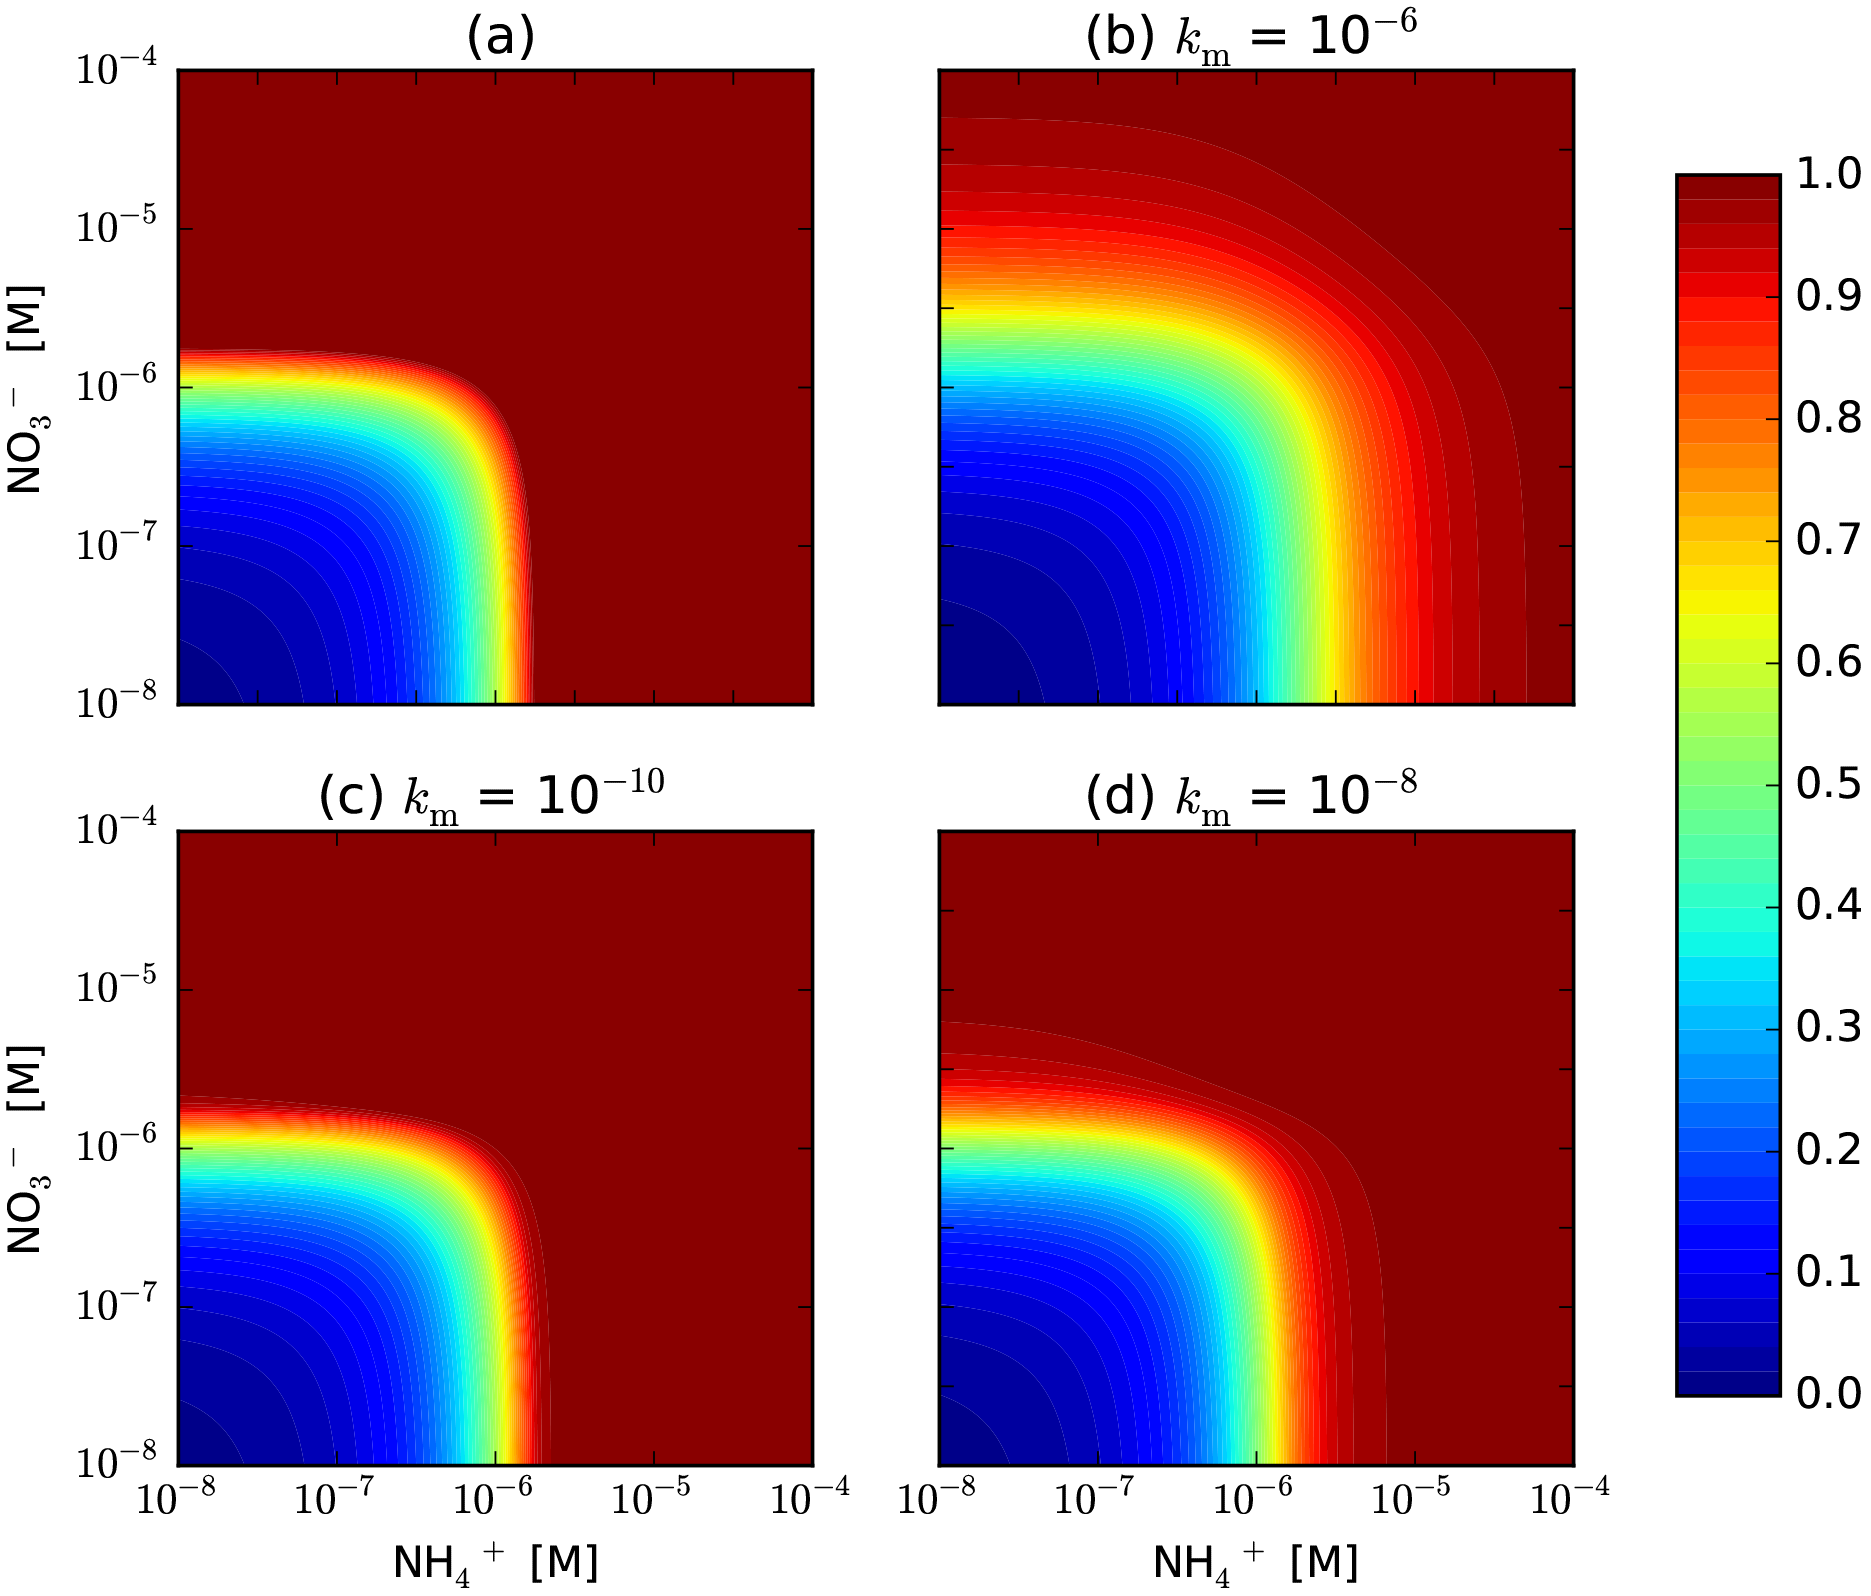
\includegraphics[width=100mm]{gmd-2015-254-f03.png}
\caption{$f_{\text{pi}}=\frac{\chem{N}_\text{take}}{\chem{N}_\text{demand}}=\max\left(1,\frac{[\chem{NH_4^+}]+[\chem{NO_3^-}]}{\chem{N}_\text{demand}}\right)$~\textbf{(a)}
vs.
$=\frac{[\chem{NH_4^+}]}{k_\mathrm{m}+[\chem{NH_4^+}]}+\left(1-\frac{[\chem{NH_4^+}]}{k_\mathrm{m}+[\chem{NH_4^+}]}\right)\frac{[\chem{NO_3^-}]}{k_\mathrm{m}+[\chem{NO_3^-}]}$~\textbf{(b--d)}
in a~0.5\,h time step with an uptake rate of 10$^{-9}$\,\unit{M\,s^{-1}}.
$f_{\text{pi}}$ for the latter representation is less than or equal to that
for the first one. The difference decreases with decreasing half saturation
$k_\mathrm{m}$.} \label{fig:demanddistribution}
\end{figure*}


\subsubsection{Nitrogen demand partitioning between ammonium and nitrate}%s3.1.3

      For comparison with CLM, we examine the uptake rate as a~function of
      demands and available concentrations $f_{\text{pi}} = ({R_\mathrm{a} +
      R_\mathrm{n}})/{R_\mathrm{p}}$ as implemented in
      Eqs.~(\ref{eq:plantarate}) and~(\ref{eq:plantnrate}).  As an example,
      we consider uptake $R_\mathrm{p}=10^{-9}$\,\unit{M\,s{^{-1}}} from
      a~solution with various [\chem{NH_4^+}] and [\chem{NO_3^-}] for
      a~0.5\,h time step. With CLM, $f_{\text{pi}}=1$ when
      $[\chem{NH_4^+}]+[\chem{NO_3^-}]\geq R_\mathrm{p}\Delta t$; otherwise,
      it decreases with decreasing [\chem{NH_4^+}]\,$+$\,[\chem{NO_3^-}]
      (Fig.~\ref{fig:demanddistribution}). The new representation
      (Eqs.~\ref{eq:plantarate} and~\ref{eq:plantnrate}) is generally
      similar, with $f_{\text{pi}}=1$ or 0 when [\chem{NH_4^+}] or
      [\chem{NO_3^-}]\,$\gg$ or $\ll k_\mathrm{m}$. For the intermediate
      concentrations, $f_{\text{pi}}$ in the new scheme is less than or
      equal to that in CLM because \chem{NH_4^+} ``inhibits'' \chem{NO_3^-}
      uptake. The difference decreases with decreasing $k_\mathrm{m}$,
      apparently disappearing at $k_\mathrm{m} = 10^{-10}$. Various levels
      of preferences of ammonium over nitrate uptake were observed for
      plants
      \citep{Pfautsch2009,Warren2007,Nordin2001,Falkengren1995,Gherardi2013},
      which is similar to microbial uptake of inorganic and organic nitrogen
      species
      \citep{Fouilland2007,Kirchman1994,Kirchman1998,Middelburg2000,Veuger2004}. CLM
      implies a~strong preference for ammonium over nitrate. For example, if
      ammonium is abundant, nitrate will not be taken by plants. The new
      scheme allows the level of preference to be adjusted by varying
      $k_\mathrm{m}$; more realistic representations can be implemented
      relatively easily.



\subsection{CLM--PFLOTRAN simulations}%s3.2

      We test the implementation by running CLM--PFLOTRAN simulations for
      Arctic (US-Brw), temperate (US-WBW), and tropical (BR-Cax) AmeriFlux
      sites. The CLM--PFLOTRAN simulations are run in the mode in which
      PFLOTRAN only handles subsurface chemistry (decomposition,
      nitrification, denitrification, plant nitrogen uptake). For comparison
      with CLM, (1)~depth and \chem{O_2} availability impact on
      decomposition, (2)~cryoturbation, (3)~SOM transport, and (4)~nitrogen
      leaching are ignored by setting (1)~decomp\_depth\_efolding to
      10$^6$\,m, o\_scalar to 1, (2)~cryoturb\_diffusion,
      (3)~som\_diffusion, and (4)~sf\_no3 and sf\_sminn to 0
      \citep{Oleson2013}. Spin-up simulations are used because they are
      numerically more challenging as the simulations start far away from
      equilibrium. In these site simulations, PFLOTRAN uses the same 10
      layer grid for the 3.8\,m one-dimensional column as CLM. The
      simulation durations are 1000, 600, and 600~years for the Arctic,
      temperate, and tropical sites, respectively.  In the base case,
      $k_\mathrm{m}=10^{-6}$\,\unit{mol\,m^{-3}} and residual concentration
      is 10$^{-15}$\,\unit{mol\,m^{-3}}. To assess the sensitivity of
      various preference levels for ammonium and nitrate uptake, and
      downregulation levels, we examine $k_\mathrm{m}=10^{-3}$ to
      $10^{-9}$\,\unit{mol\,m^{-3}}. We evaluate how scaling, clipping, and
      log transformation for avoiding negative concentrations influence
      accuracy and efficiency.  The simulations are conducted using the ORNL
      Institutional Cluster (OIC Phase5, an SGI Altix with dual 8-core AMD
      Opterons per compute node) with CLM--PFLOTRAN (as well as third-party
      libraries MPICH, PETSc, NetCDF, HDF5, etc.) compiled with gfortran
      4.8.1 with the ``-O1'' optimization level.  Due to the small size of
      the simulations, our tests use only a~single CPU core.

%f4
\begin{figure*}[t]
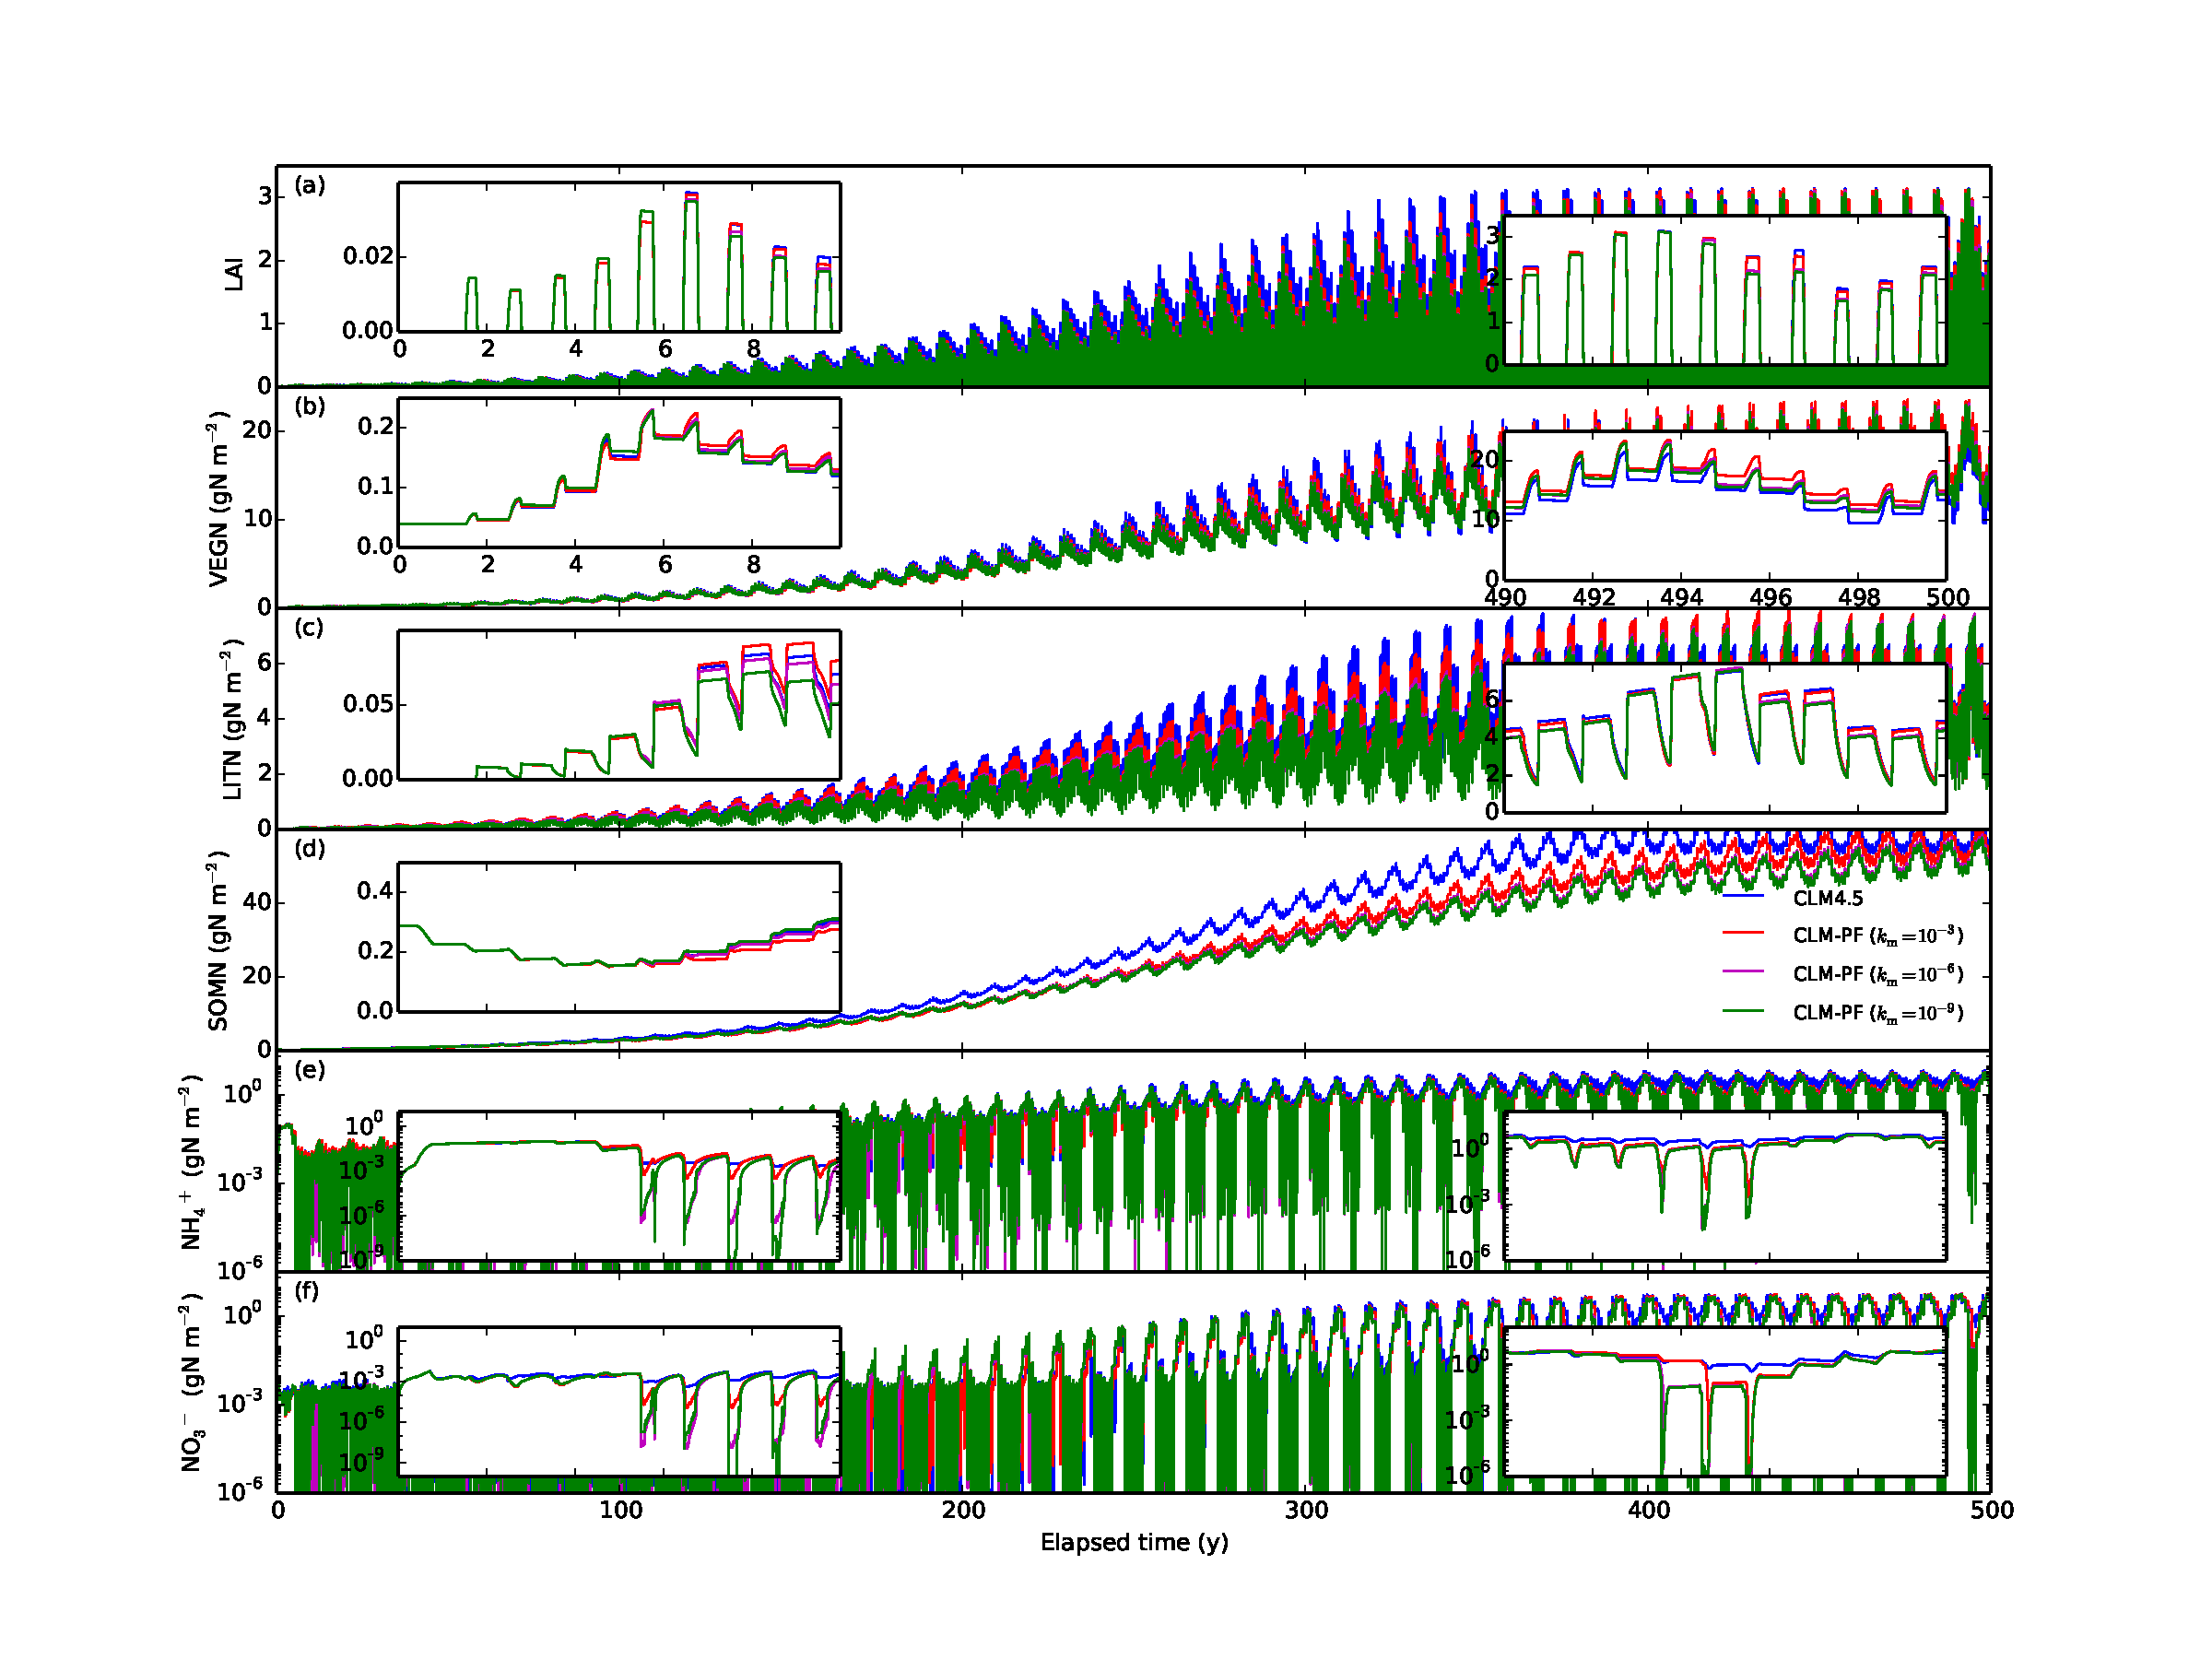
\includegraphics[width=130mm]{gmd-2015-254-f04.pdf}
\caption{Calculated LAI and nitrogen distribution among vegetation, litter,
SOM, \chem{NH_4^+}, and \chem{NO_3^-} pools in spin-up simulations for the
US-Brw site.} \label{fig:brw500yl}
\end{figure*}


\subsubsection{Site descriptions}%s3.2.1

      The US-Brw site (71.35{\degree}\,N, 156.62{\degree}\,W) is located
      near Barrow, Alaska. The mean annual temperature, precipitation, and
      snowfall are $-12$\,\unit{\degree C}, 11\,\unit{cm}, and
      69\,\unit{cm}, respectively (1971--2000) \citep{Lara2012}. The
      landscape is poorly drained polygonized tundra. The maximum thaw depth
      ranges from 30 to 40\,\unit{cm}, and the snow-free period is variable
      in length but generally begins in early June and lasts until early
      September \citep{Hinkel2003}. The area is composed of several
      different representative wet--moist coastal sedge tundra types,
      including wet sedges, grasses, moss, and assorted lichens. The leaf
      area index (LAI) is $\sim 1.1$ (AmeriFlux data).

      The US-WBW site (35.96{\degree}\,N, 84.29{\degree}\,W) is located in
      the Walker Branch Watershed in Oak Ridge, Tennessee
      \citep{Hanson2003}. The climate is typical of the humid southern
      Appalachian region. The mean annual precipitation is $\sim
      139$\,\unit{cm}, and the mean median temperature is
      14.5\,\unit{\degree C}.  The soil is primarily Ultisols that developed
      in humid climates in the temperate zone on old or highly weathered
      material under forest. The temperate deciduous broadleaf forest was
      regenerated from agricultural land 50~years ago.  LAI is $\sim 6.2$
      \citep{Hanson2004}.

      The BR-Cax site ($-$1.72{\degree}\,N, $-$51.46{\degree}\,W) is located
      in the eastern Amazon tropical rainforest. The mean annual rainfall is
      between 200 and 250\,\unit{cm}, with a~pronounced dry season between
      June and November. The soil is a~yellow Oxisol (Brazilian
      classification \textit{Latossolo Amarelo}) with a~thick stony laterite layer at
      3--4\,m depth \citep{daCosta2010}. The vegetation is evergreen
      broadleaf forest. The LAI is $\sim$ 4--6 \citep{Powell2013}.



\subsubsection{CLM--PFLOTRAN site simulation results}%s3.2.2


      The site climate data from 1998 to 2006, 2002 to 2010, and 2001 to
      2006 are used to drive the spin-up simulation for the Arctic (US-Brw),
      temperate (US-WBW), and tropical (BR-Cax) sites, respectively. This
      introduces a~multi-year cycle in addition to the annual cycle
      (Figs.~\ref{fig:brw500yl}--\ref{fig:cax300yl}). Overall, CLM--PFLOTRAN
      is close to CLM4.5 in predicting LAI and nitrogen distribution among
      vegetation, litter, SOM (soil organic matter), ammonium and nitrate
      pools for the Arctic (Fig.~\ref{fig:brw500yl}), temperate
      (Fig.~\ref{fig:pit300yl}), and tropical (Fig.~\ref{fig:cax300yl})
      sites. CLM4.5 does reach equilibrium earlier than CLM--PFLOTRAN. The
      maximum differences occur during the transient periods (200--400~years
      for the Arctic, and 50--70~years for the temperate and tropical
      sites) for \chem{SOMN} (soil organic matter nitrogen), ammonium, and
      nitrate. This is not surprising as (1)~the nitrogen demand competition
      scheme implemented in CLM--PFLOTRAN is different from that in CLM4.5
      (Fig.~\ref{fig:demanddistribution}), (2)~the former solves the
      reaction network simultaneously while the latter does so sequentially
      (resolve the plant uptake and decomposition first, then nitrification,
      then denitrification), and (3)~the carbon nitrogen cycle is very
      sensitive to the nitrogen competition representation. Close to steady
      state, both CLM4.5 and CLM--PFLOTRAN overpredict the LAI at the Arctic
      and temperate sites, and underpredict soil organic matter
      accumulation, which will be resolved in future work.

%f5
\begin{figure*}[t]
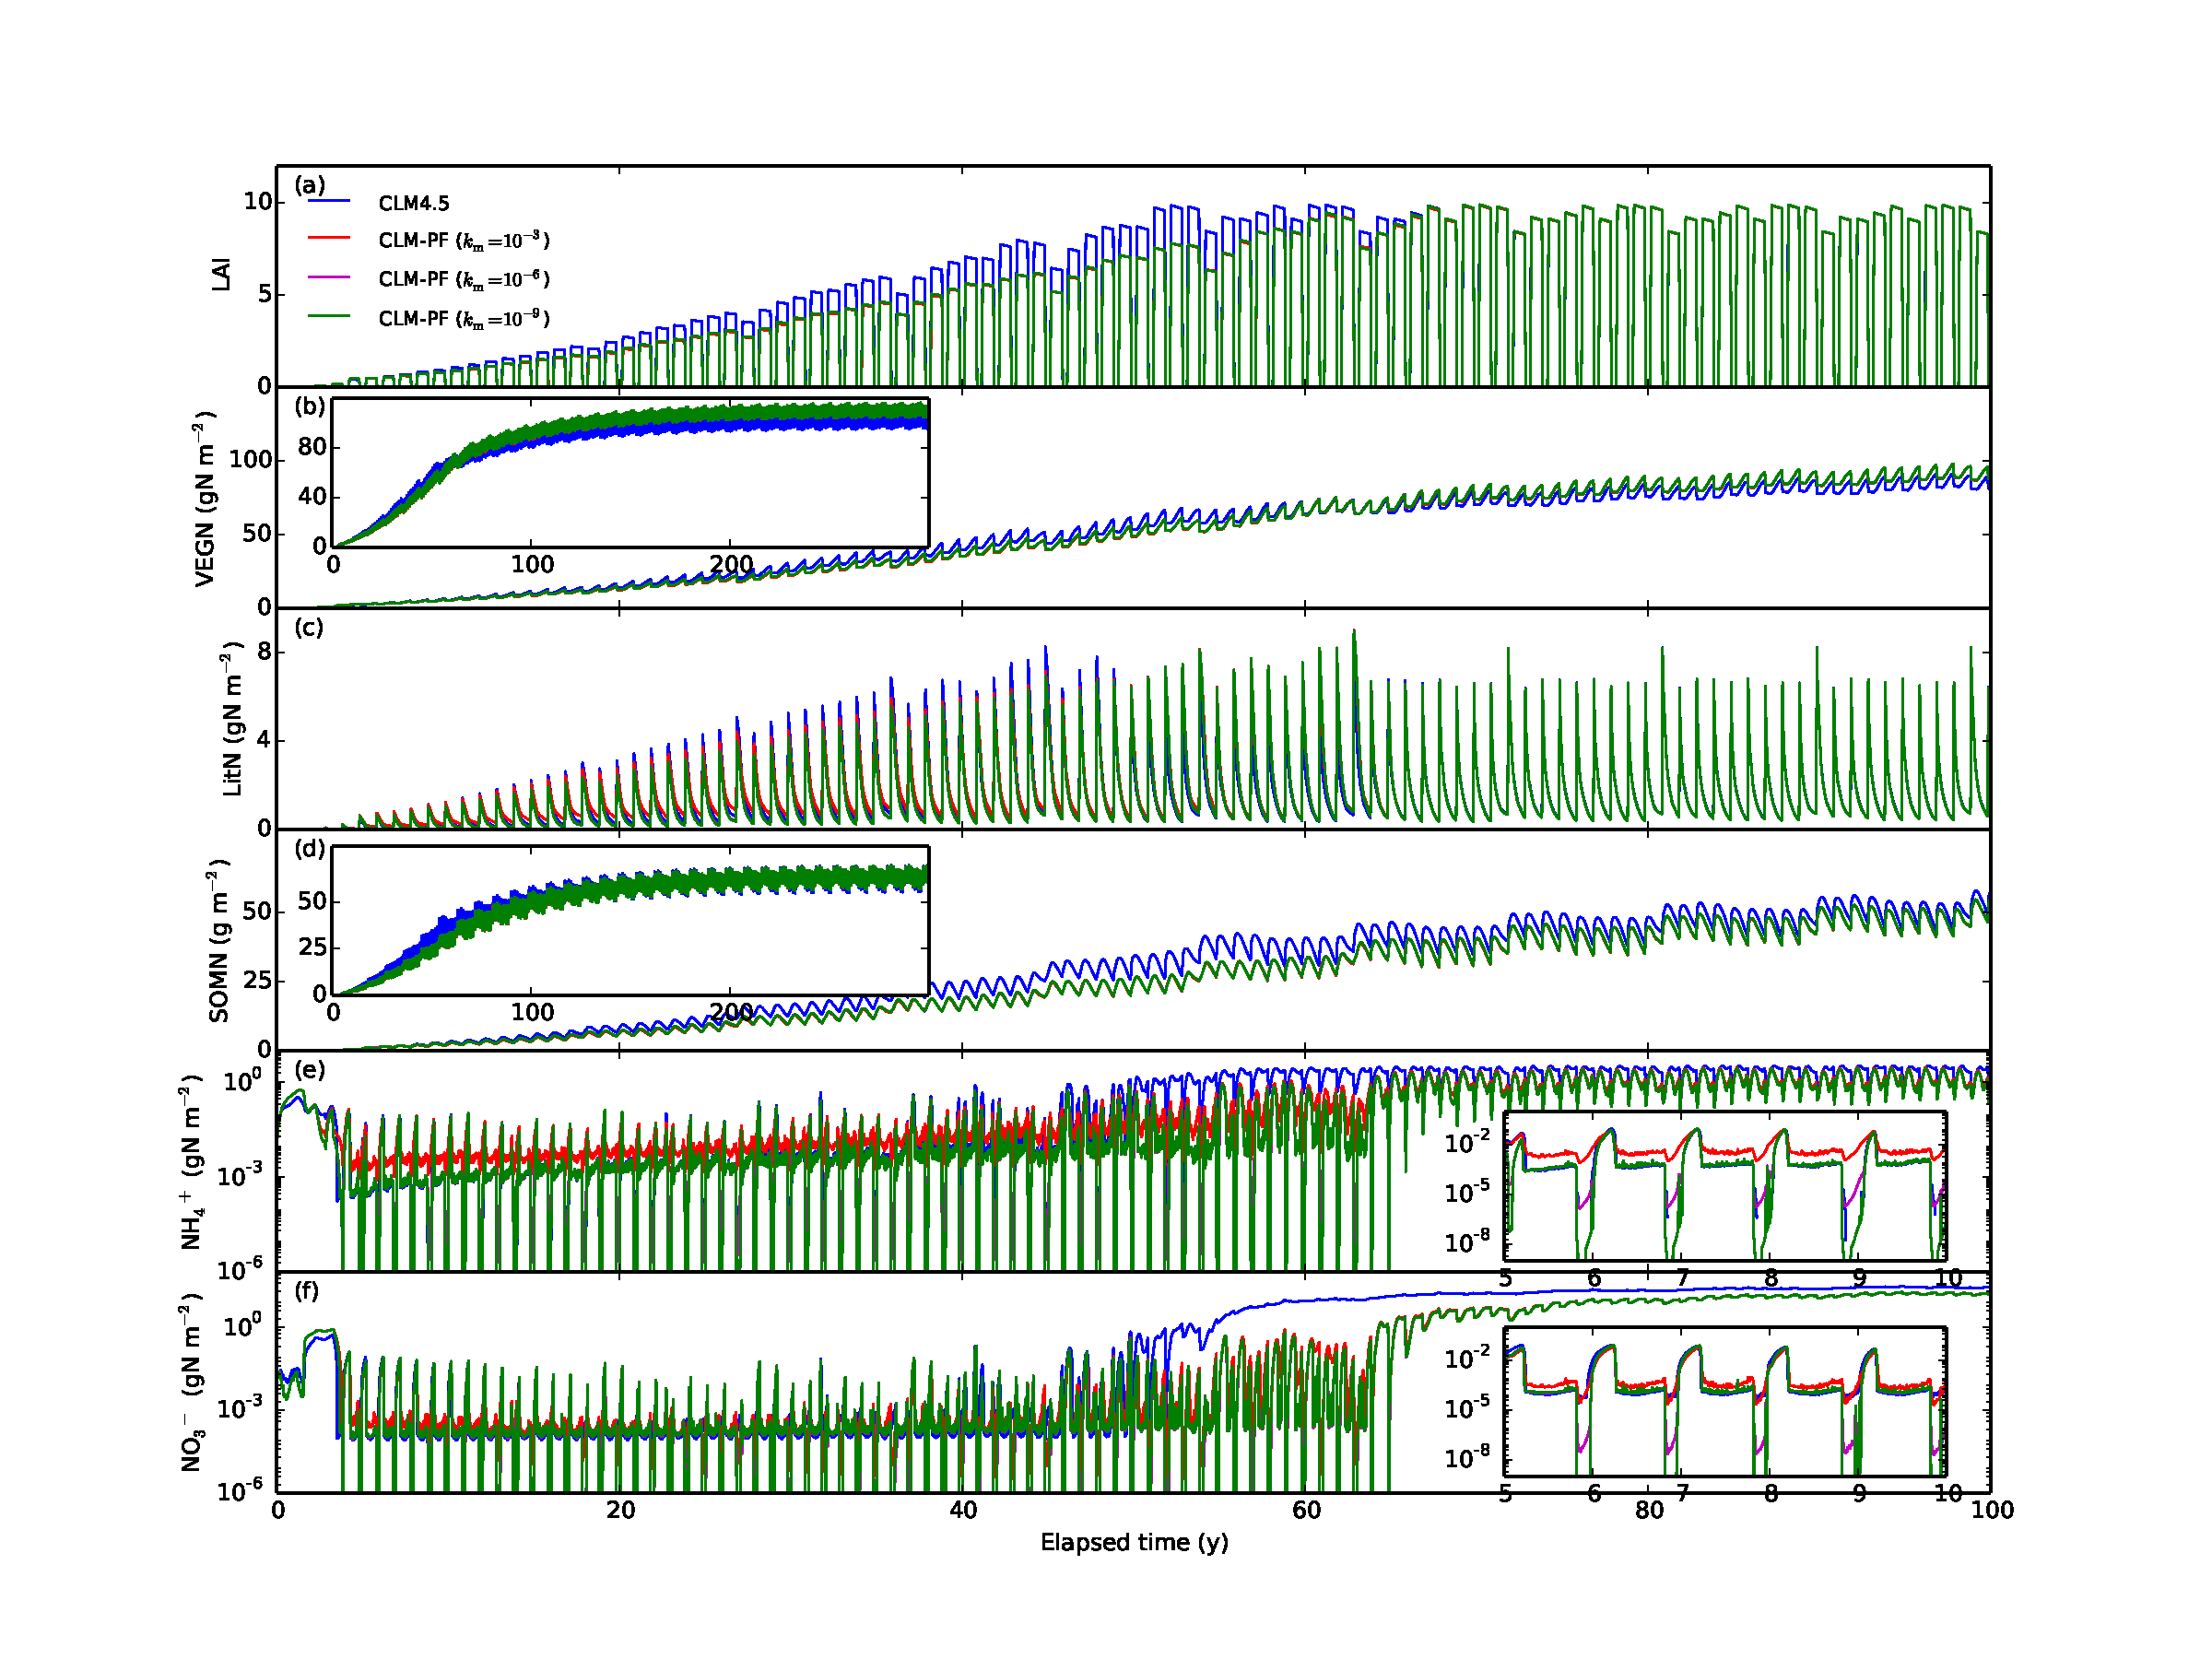
\includegraphics[width=130mm]{gmd-2015-254-f05.pdf}
\caption{Calculated LAI and nitrogen distribution among vegetation, litter,
SOM, \chem{NH_4^+}, and \chem{NO_3^-} pools in spin-up simulations for US-WBW
site.} \label{fig:pit300yl}
\end{figure*}


      The Arctic site shows a~distinct summer growing season
      (Fig.~\ref{fig:brw500yl}): LAI and VEGN (vegetation nitrogen) jump up
      at the beginning, then level off, and drop down at the end of the
      growing season when LITN (litter nitrogen) jumps up due to litter
      fall.  Ammonium and nitrate concentrations drop to very low levels at
      the beginning of the growing season and accumulate at other times. In
      addition to a~longer growing season than the Arctic site, the
      temperate site shows more litter fall by the end of the growing
      season, as it is a~temperate deciduous forest, which introduces
      immobilization demand that further lowers ammonium and nitrate
      concentrations (Fig.~\ref{fig:pit300yl}e inset). The seasonality is
      much less apparent in the tropical site than in the Arctic and
      temperate sites. LAI, VEGN, LITN, and SOMN accumulate with less
      seasonal variation to reach equilibrium.

      The higher $k_\mathrm{m}$ of
      $10^{-3}$\,\unit{mol\,m^{-3}} results in lower immobilization, higher
      accumulation of LITN, and higher ammonium and nitrate concentrations
      than $k_\mathrm{m}$ of $10^{-6}$\,\unit{mol\,m^{-3}} for the tropical site
      during the spin-up (Fig.~\ref{fig:cax300yl}). This is not surprising becasue
      a higher $k_\mathrm{m}$ of $10^{-3}$\,\unit{mol\,m^{-3}} numerically poses
      a stricter limitation on the extent that plants and microbes can take from soils.
      The range of
      $k_\mathrm{m}$ values (10$^{-6}$, and 10$^{-9}$\,\unit{mol\,m^{-3}})
      generally has limited impact on the overall calculations except that
      the nitrogen concentrations drop lower with lower $k_\mathrm{m}$
      values (e.g., inset in Figs.~\ref{fig:brw500yl}e~and~f
      and~\ref{fig:pit300yl}e). The lack of sensitivity is because these
      very low concentrations do not make up a~mass of nitrogen that is
      significant enough to influence the carbon and nitrogen cycle.
      However, as a~small $k_\mathrm{m}$ means low concentrations (test 4),
      and weak downregulation and steep transition between zero order and
      first order, it has implications on accuracy and efficiency of the
      numerical solutions.



\subsubsection{Accuracy and efficiency}%s3.2.3

      Numerical errors introduced due to false convergence in clipping,
      scaling, or log transformation are captured in CLM when it checks
      carbon and nitrogen mass balance for every time step for each column,
      and reports $\geq 10^{-8}$\,\unit{g\,m^{-2}} errors (to reduce log file size as the simulation durations are hundreds of years and the time-step size is half an hour).  When log
      transformation is used, mass balance errors are not reported for the
      Arctic, temperate, and tropical sites with $k_\mathrm{m}$ values
      10$^{-3}$, 10$^{-6}$, and 10$^{-9}$\,\unit{mol\,m^{-3}}. The computing
      time for CLM--PFLOTRAN is about 60--100\,{\%} more than that of
      CLM (Table~\ref{tab:computingtime}). This is not unreasonably high as
      the implicit method involves solving a~Jacobian system for each
      Newton--Raphson step (Eq.~\ref{eq:axb}), and log transformation
      converts the linear problem into a~nonlinear one. The computational
      cost increases substantially with decreasing half saturation, which is
      expected as a~smaller half saturation requires smaller time-step sizes
      to march through steeper transition between the zero- and first-order
      rate in Monod function. Overall, log transformation is accurate,
      robust, and reasonably efficient.


%t1
\begin{table*}[t]
\caption{Wall time for CLM--PFLOTRAN relative to CLM for spin-up simulation on
OIC (ORNL Institutional Cluster Phase5).} \label{tab:computingtime}
%\scalebox{.7}[.7]{%
\begin{tabular}{p{20mm}llp{15mm}llp{15mm}lll}
\tophline
Site &\multicolumn{3}{l}{Clipping}  &\multicolumn{3}{l}{Scaling} &\multicolumn{3}{l}{Log transformation} \\
\middlehline
$k_\mathrm{m}$ &$10^{-3}$ &$10^{-6}$ &$10^{-9}$ &$10^{-3}$ &$10^{-6}$ &$10^{-9}$ &$10^{-3}$ &$10^{-6}$ &$10^{-9}$\\
\cline{1-10}
US-Brw &1.28      &1.30 &1.30 &1.29 &1.29 &1.32 &1.45 &1.49 &1.72 \\
US-WBW   &1.45    &1.47 &1.47 &1.45 &1.45 &1.47 &1.64 &1.68 &1.89 \\
BR-Cax &1.43      &1.49 &1.55 &1.44 &1.48 &1.52 &1.62 &1.66 &1.99 \\
\bottomhline
\end{tabular}
%}
%\hack{\setlength\tabularwidth{0.7142\tabularwidth}}%
%\scalebox{.7}[.7]{%
\belowtable{%
%\hack{\vspace*{2mm}}%        <-- aber NUR bei Verkleinerungsfaktor notwendig !!
CLM wall time is 29.3, 17.7, and 17.1\,h for the Arctic, temperate, and
tropical sites for a~simulation duration of 1000, 600, and 600~years.
$k_\mathrm{m}$ is the half saturation (mol\,m$^{-3}$). }
%}
\end{table*}

      Mass balance errors are reported for $k_\mathrm{m}$ values of
      10$^{-6}$, and 10$^{-9}$ but not for 10$^{-3}$\,\unit{mol\,m^{-3}}
      when clipping is applied.  With $k_\mathrm{m} =
      10^{-3}$\,\unit{mol\,m^{-3}}, the plant uptake and immobilization are
      inhibited at relatively high concentration so that nitrogen
      concentrations are high. With $k_\mathrm{m}$ decreasing from 10$^{-6}$
      to 10$^{-9}$\,\unit{mol\,m^{-3}}, nitrogen concentrations are lowered
      to a~much lower level (Figs.~\ref{fig:brw500yl}--\ref{fig:cax300yl},
      similar to Fig.~\ref{fig:decomp}c), increasing the likelihood of
      overshoot.  Mass balance errors are reported when the relative update
      is below STOL, preventing further iterations from resolving the
      violation of reaction stoichiometry introduced by clipping. The
      frequency of mass balance errors decreases with increasing
      $k_\mathrm{m}$, and decreasing STOL. Tightening STOL from 10$^{-8}$ to
      10$^{-12}$, the reported greater than 10$^{-8}$\,\unit{g\,m^{-3}} mass
      balance errors are eliminated. The computing time is about 50\,{\%}
      more than CLM, which is more efficient than log transformation
      (Table~\ref{tab:computingtime}), particularly for
      $k_\mathrm{m}=10^{-9}$\,\unit{mol\,m^{-3}}. Tightening STOL only
      slightly increases the computing time. Because clipping often occurs
      at very low concentrations, the reported mass balance errors are
      usually small ($\sim 10 ^{-8}$\,\unit{g\,N\,m^{-2}} to $\sim 10
      ^{-7}$\,\unit{g\,N\,m^{-2}}), and do not have substantial impact on
      the overall simulation results.


%f6
\begin{figure*}
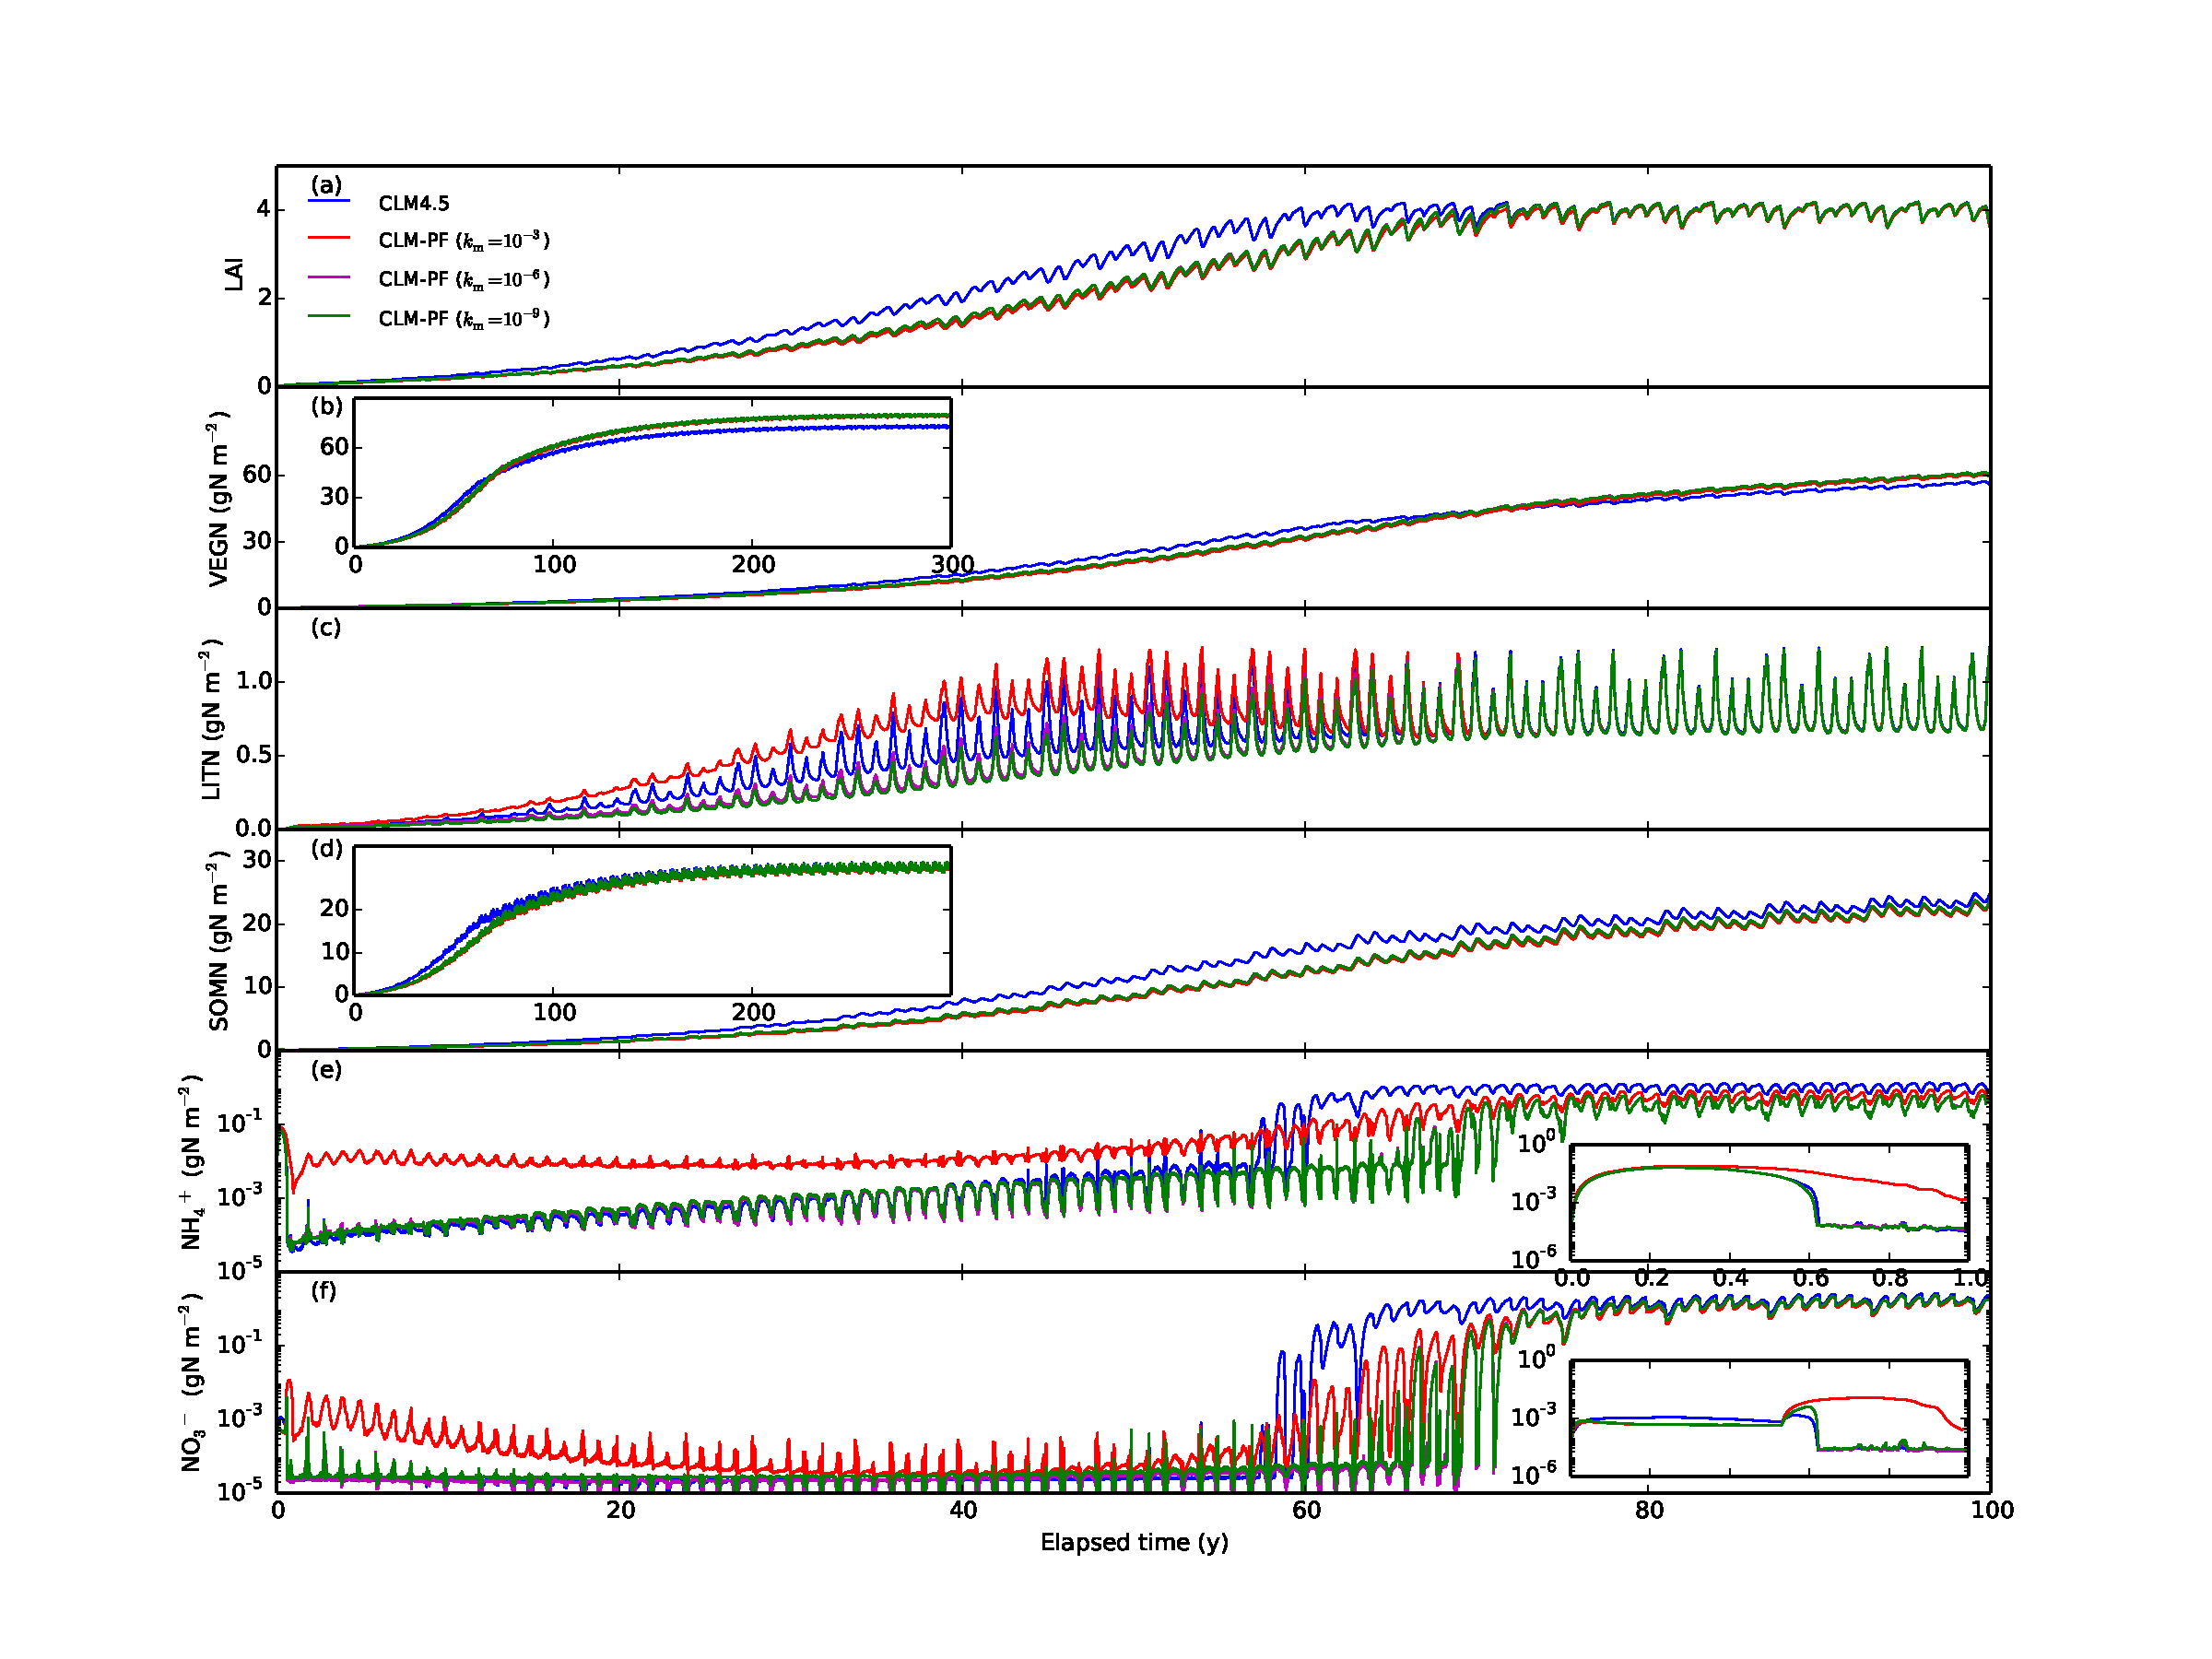
\includegraphics[width=130mm]{gmd-2015-254-f06.pdf}
\caption{Calculated LAI and nitrogen distribution among vegetation, litter,
SOM, \chem{NH_4^+}, and \chem{NO_3^-} pools in spin-up simulations for BR-Cax
site.} \label{fig:cax300yl}
\end{figure*}

%f7
\begin{figure}[p]
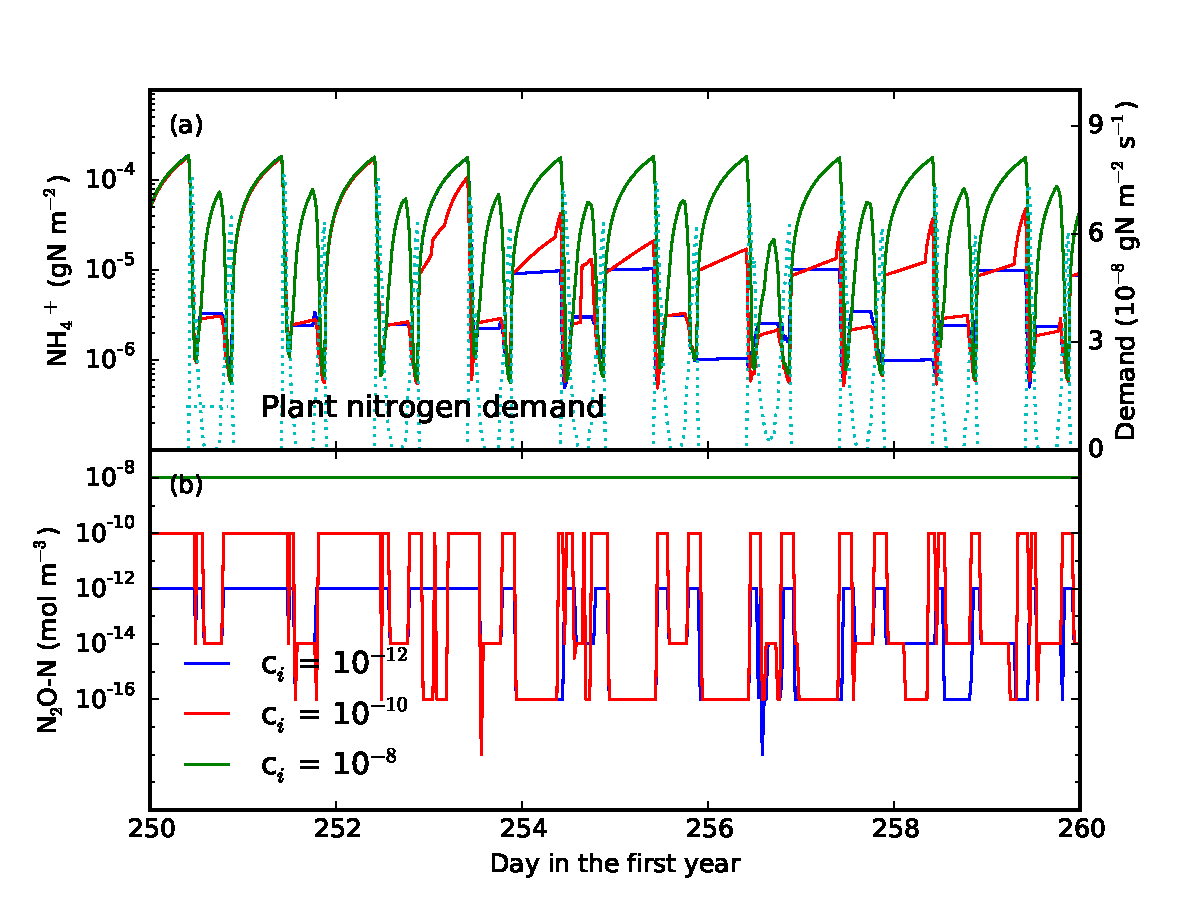
\includegraphics[width=85mm]{gmd-2015-254-f07.pdf}
\caption{Resetting nitrous oxide concentration to $10^{-8}$, $10^{-10}$, and
$10^{-12}$\,\unit{mol\,m^{-3}} in every CLM 0.5\,h time-step results in no
inhibition to increasing inhibition of reactions when the scaling method is
used with STOL\,$=$\,$10^{-8}$. \chem{N_2O-N} concentration in the $y$~axis
in~\textbf{(b)} is the minimum of the 10 soil layers. Numerical experiments
are conducted for the tropical site for the first year with
$k_\mathrm{m}=10^{-6}$\,\unit{mol\,m^{-3}}. See inset in
Fig.~\ref{fig:cax300yl}e for ammonium concentration in the first year with
daily data points.} \label{fig:cax1yn2o}
\end{figure}



      The results for scaling is similar to clipping: mass balance errors
      are reported for $k_\mathrm{m}$ values of 10$^{-6}$ and 10$^{-9}$ but
      not for 10$^{-3}$\,\unit{mol\,m^{-3}}; tightening STOL to $10^{-12}$
      eliminates these errors; it takes about 50\,{\%} more computing time
      than CLM. To examine the influence of low concentrations on the
      accuracy and efficiency of the scaling method, we conduct numerical
      experiments in which we reset the nitrous oxide concentration produced
      from decomposition (Reaction~\ref{rxn:nitr2n2o}, rate
      Eq.~\ref{eq:nitr2n2odecomp}) to 10$^{-12}$, 10$^{-10}$, or
      10$^{-8}$\,\unit{mol\,m^{-3}} in each CLM half-hour time step for the
      tropical site for the first year. This can be used to calculate the
      nitrous oxide production rate from decomposition and feed back to CLM
      without saving the concentration for the previous time step. Overall,
      nitrogen is abundant in the first half year, and then becomes limiting
      in the last 5 months (Fig.~\ref{fig:cax300yl}e~and~f, inset). We
      look into the daily ammonium cycles as an example during the nitrogen-limiting period (day 250 to 260, Fig.~\ref{fig:cax1yn2o}a). Every day
      the ammonium concentration increases with time due to deposition, but
      drops when the plant nitrogen demand shots up. With a~reset
      concentration of $10^{-8}$\,\unit{mol\,m^{-3}}, the minimum nitrous
      oxide concentration for the 10 layers is
      $10^{-8}$\,\unit{mol\,m^{-3}}, and ammonium concentrations show two
      peaks followed by two drops due to the two plant uptake peaks every
      day. Decreasing the reset concentration to
      $10^{-10}$\,\unit{mol\,m^{-3}}, the minimum concentration drops to
      $10^{-12}$, $10^{-14}$, and $10^{-16}$\,\unit{mol\,m^{-3}},
      corresponding to 1, 2, and 3 scaling iterations with overshoot for
      nitrous oxide. These result in numerical ``inhibition'' of nitrogen
      rebound every day. It worsens with further decrease of the reset
      concentration to $10^{-12}$\,\unit{mol\,m^{-3}}. This introduces mass
      balance errors as reported in CLM because the false convergence
      numerically inhibits all of the reactions including nitrogen
      deposition and litter input from CLM to PFLOTRAN.  Unlike clipping,
      these false convergences introduce excessive mass balance errors
      because of the inhibition of productions specified from CLM. If all of
      the reactions are internally balanced, false convergence does not
      result in mass balance errors.

%f8
\begin{figure}[t]
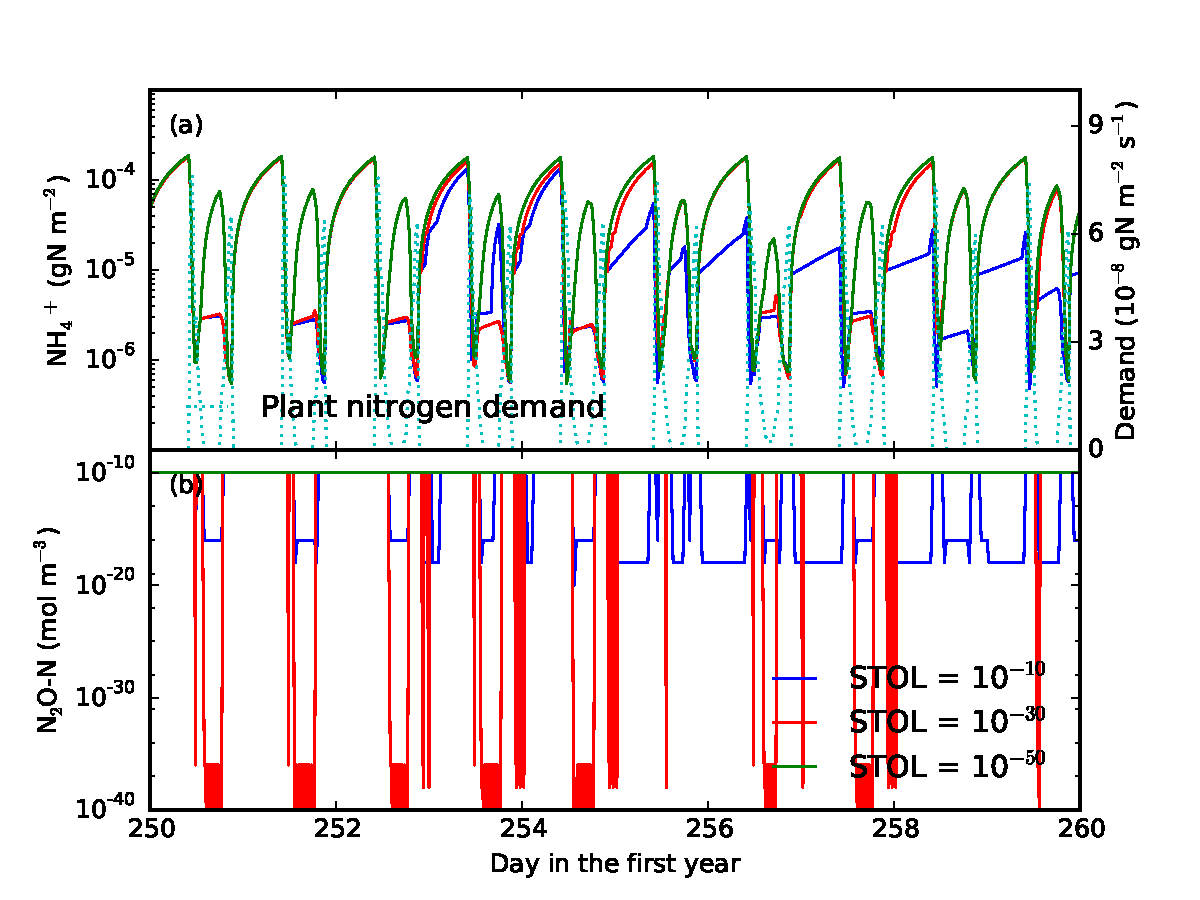
\includegraphics[width=85mm]{gmd-2015-254-f08.pdf}
\caption{Decreasing STOL can decrease and eliminate the numerical inhibition
in the case of $c_i = 10^{-10}$\,\unit{mol\,m^{-3}} in
Fig.~\ref{fig:cax1yn2o}. \chem{N_2O-N} concentration in the $y$~axis
in~\textbf{(b)}
 is the minimum of the 10 soil layers.}
\label{fig:cax1yn2osto0}
\end{figure}


      The frequent negative update to nitrous oxide is produced because the
      rate for the nitrification Reaction~(\ref{rxn:nitr2n2o}) is
      parameterized as a~fraction of the net nitrogen mineralization rate to
      reflect the relationship between labile carbon content and nitrous
      oxide production \citep{Parton1996}. A~Monod function is added to
      describe the limitation of ammonium concentration on nitrification.
      Calculation of the net mineralization rate involves all of the
      decomposition reactions, and the litter decomposition reactions bring
      in ammonium and nitrate limitation, and ammonium inhibition on nitrate
      immobilization. As a~result, the off-diagonal terms for nitrous oxide
      in the Jacobian matrix corresponding to \chem{Lit1C}, \chem{Lit1N},
      \chem{Lit2C}, \chem{Lit2N}, \chem{Lit3C}, \chem{Lit3N}, \chem{SOM1},
      \chem{SOM2}, \chem{SOM3}, \chem{SOM4}, ammonium, and nitrate are
      nonzero. Negative updates to all of these species contribute to
      negative updates to nitrous oxide. Similar to tests 2--3, a~negative
      update to a~low nitrous oxide concentration can decrease
      $\text{snorm}_{\text{rel}}$ to below STOL, resulting in false
      convergence and mass balance errors. While the empirical
      parameterization of nitrification rate as a~function of net
      mineralization rate is conceptually convenient, it increases the
      complexity of the reaction network and computational cost due to the
      reduced sparsity of the Jacobian matrix. While we use nitrous oxide as
      an example here, similar results can be obtained for \chem{PlantN},
      \chem{PlantA}, and nitrogen gas produced from denitrification,
      etc. Theoretically, the numerical ``inhibition'' of all reactions can
      be caused by negative updates to very low concentrations for any
      species.

      The numerical errors can be decreased and eliminated by decreasing
      STOL.  Similar to the tests 2--3 a
      small STOL can result in small $\text{snorm}_{\text{rel}}$, then
      a~very small STOL is needed. For the case of reset concentration
      10$^{-10}$ for the 1 year tropical site simulation, the numerical
      ``inhibition'' decreases with decreasing STOL and varnishes for the
      observed time window when STOL\,$=$\,$10^{-50}$
      (Fig.~\ref{fig:cax1yn2osto0}), indicating the need for very small,
      zero, or even negative STOL to avoid false convergence. The impact of
      resetting nitrous oxide concentration on clipping and log
      transformation is less dramatic. Nevertheless, the computing time
      increases about 10\,{\%} for clipping, and doubles for the log
      transformation.



\conclusions[Summary and conclusions]

      Global land surface models have traditionally represented subsurface
      soil biogeochemical processes using preconfigured reaction
      networks. This hardcoded approach makes it necessary to revise source
      code to test alternative models or to incorporate improved process
      understanding. We couple PFLOTRAN with CLM to facilitate testing of
      alternative models and incorporation of new understanding. We
      implement CLM-CN decomposition cascade, nitrification,
      denitrification, and plant nitrogen uptake reactions in
      CLM--PFLOTRAN. We illustrate that with implicit time stepping using the
      Newton--Raphson method, the concentration can become negative during
      the iterations even for species that have no consumption, which need
      to be prevented by intervening in the Newton--Raphson iteration
      procedure.

      Simply stopping the iteration with negative concentration and
      returning to the time-stepping subroutine to cut time-step size can
      avoid negative concentration, but may result in small time-step sizes
      and high computational cost. Clipping, scaling, and log transformation
      can all prevent negative concentration and reduce computational
      cost but at the risk of accuracy. Our results reveal implications when the relative update
      tolerance (STOL) is used as one of the convergence criteria. While use
      of STOL improves efficiency in many situations, satisfying STOL does
      not guarantee satisfying the residual equation, and therefore it may
      introduce false convergence. Clipping reduces the consumption but not
      the production in some reactions, violating reaction
      stoichiometry. Subsequent iterations are required to resolve this
      violation. A~tight STOL is needed to avoid false convergence and
      prevent mass balance errors. While the scaling method reduces the
      whole update vector following the stoichiometry of the reactions to
      maintain mass balance, a~small scaling factor caused by a~negative
      update to a~small concentration may diminish the update and result in
      false convergence, numerically inhibiting all reactions, which is not
      intended for productions with external sources (e.g., nitrogen
      deposition from CLM to PFLOTRAN). For accuracy and efficiency, a~very
      tight STOL is needed when the concentration can be very low. Log
      transformation is accurate and robust, but requires more computing
      time. The computational cost increases with decreasing concentrations,
      most substantially for log transformation.

      These computational issues arise because we switch from the explicit
methods to the implicit methods for soil biogeochemistry. We use small half
saturation (e.g., 10$^{-9}$), residual concentration (e.g., 10$^{-15}$,
slightly above machine zero), and large initial time-step size (e.g., 0.5\,h)
to exemplify the causes of the accuracy, efficiency, and robustness issues.
For the zero-order rate formulae in CLM, the limitation of reactant (nitrogen
in this work) availability needs to be explicitly represented for robustness
and flexibility. With mechanistic representations, reaction stops or reverses
when the rate-limiting reactants decrease to a threshold, or when the
reaction becomes thermodynamically unfavorable, nullifying the need for half
saturation and residual concentration. Before our representations are
sufficiently mechanistic, a small residual concentration (say 10$^{-15}$)
serves as a safeguard to avoid failure for the log transformation method and
unnecessary efficiency and accuracy loss for the clipping and scaling methods
unless a smaller residual concentration is dictated by physical and chemical
conditions.

For reactions with very low half saturation and residual concentrations, e.g.,
redox reactions involving O$_2$, H$_2$, and CH$_4$, STOL
can be set to zero to avoid false convergence, at the risk of potential
increased computational cost. Increasing STOL (say to 10$^{-12}$) decreases
computing time at the risk of potential accuracy loss. To cover a wide range of
many orders of magnitude concentrations in soil biogeochemistry and for
accuracy and robustness, the modelers can start with the log transformation
method. If it is desirable to reduce the computational time, STOL can be
relaxed, and clipping can be used without log transformation. The scaling
method is another option but with strict STOL requirement. As the accuracy is
checked and logged in CLM for carbon and nitrogen mass balance, the modelers
can assess the tradeoff between efficiency and accuracy in CLM--PFLOTRAN and
select their optimum.

            Our CLM--PFLOTRAN spin-up simulations at Arctic, temperate, and
      tropical sites produce results similar to CLM4.5, and indicate that
      accurate and robust solutions can be achieved with clipping, scaling, or
      log transformation. The computing time is 50 to 100\,{\%} more than
      CLM4.5 for a~range of half saturation values from 10$^{-3}$ to
      10$^{-9}$ and a~residual concentration of 10$^{-15}$ for nitrogen. As
      physical half saturation ranges from 10$^{-5}$ to 10$^{-6}$\,\unit{M}
      for nitrogen, and the detection limits are often above
      10$^{-9}$\,\unit{M}, our results indicate that accurate, efficient,
      and robust solutions for current CLM soil biogeochemistry can be
      achieved using CLM--PFLOTRAN.  We thus demonstrate the feasibility of
      using an open-source, general-purpose reactive transport code with
      CLM, enabling significantly more complicated and more mechanistic
      biogeochemical reaction systems.

      An alternative to our approach of coupling LSMs with reactive
      transport codes is to code the solution to the advection, diffusion,
      and reaction equations directly in the LSM. This has been done using
      explicit time stepping and operator splitting to simulate the
      transport and transformation of carbon, nitrogen, and other species in
      CLM \citep{Tang2013b}. An advantage of our approach of using
      a~community RTM to solve the advection--dispersion--reaction system is
      that the significant advances that the RTM community has made in the
      past several decades can be leveraged to better represent the
      geochemical processes (e.g., pH, pE) in a~systematic, flexible, and
      numerically reliable way. Given that a~wide range of conditions may be
      encountered in any one global LSM simulation, it is particularly
      important to have robust solution methods such as fully implicit
      coupling of the advection--dispersion--reaction equations \citep{Yeh1989,Zheng2002,Steefel2015}.  As a~next
      step, we hope CLM--PFLOTRAN will facilitate investigation of the role
      of the redox sensitive microbial reactions for methane production and
      consumption, and nitrification and denitrification reactions in
      ecological responses to climate change.

\hack{\newpage}
\subsection*{Code availability}
PFLOTRAN is open-source
      software. It is distributed under the terms of the GNU Lesser General
      Public License as published by the Free Software Foundation either
      version 2.1 of the License, or any later version. It is available at
      \url{https://bitbucket.org/pflotran}. CLM--PFLOTRAN is under
      development and will be made available according to the NGEE-Arctic
      Data Management Policies and Plans
      (\url{http://ngee-arctic.ornl.gov/content/ngee-arctic-data-management-policies-and-plans}).
      Before it becomes publicly available, please contact the corresponding
      authors to obtain access to the code.



\hack{\clearpage}

\appendix

\section{CLM biogeochemical reactions and rates}%sAA
\label{sec:clmbgc}


\subsection{CLM-CN decomposition}%sAA1
\label{section:bgc}

      The CLM-CN decomposition cascade consists of three litter pools with
      variable CN ratios, four soil organic matter (SOM) pools with constant
      CN ratios, and seven reactions
      \citep{Bonan2012,Oleson2013,Thornton2005}. The reaction can be
      described by
%\hack{\arraycolsep0pt}
\begin{reaction}
\chem{CN_u} \rightarrow (1 - f) \chem{CN_d} + f \chem{CO_2} + n \chem{N},
\label{rxn:decomp}
\end{reaction}%R1
      where \chem{CN_u} and \chem{CN_d} are the upstream and downstream pools
      (molecular formula, for 1\,mol upstream and downstream pool, there is
      u and d mol\,N), \chem{N} is either \chem{NH_4^+} or \chem{NO_3^-},
      $f$ is the respiration fraction, and $n=\mathrm{u} -
      (1-f)\mathrm{d}$. The rate is
\begin{align}
 &
\frac{\mathrm{d} \chem{[CN_u]}}{\mathrm{d} t} =
- k_{d} f_{T} f_{w} \chem{[CN_u]},
\label{eq:decomprate}
\end{align}%eA1
      where $k_{d}$ is the rate coefficient, and $f_{T}$ and $f_{w}$ are
      the temperature and moisture response functions.  With a~constant CN
      ratio, the decomposition reactions for the four SOM pools are
{\hack{\arraycolsep0pt}}%
\begin{rxnarray}
& \chem{SOM1} \rightarrow 0.72 \chem{SOM2} + 0.28 \chem{CO_2} + 0.02
\chem{N}, \label{rxn:som1}
\\
& \chem{SOM2} \rightarrow 0.54 \chem{SOM3} + 0.46 \chem{CO_2} + 0.025143
\chem{N}, \label{rxn:som2}
\\
& \chem{SOM3} \rightarrow 0.45 \chem{SOM4} + 0.55 \chem{CO_2} + 0.047143
\chem{N}, \label{rxn:som3}
\end{rxnarray}%R2 -- R4
      and
\begin{reaction}
\chem{SOM4} \rightarrow \chem{CO_2} + 0.085714 \chem{N}.
\label{rxn:som4}
\end{reaction}%R5
      The exact stoichiometric coefficients are calculated in the code using
      values for respiration factor, CN ratio, and molecular weight
      specified in the input file.

      CLM4.5 has an option to separate \chem{N} into \chem{NH_4^+} and
      \chem{NO_3^-}.  The \chem{N} mineralization product is \chem{NH_4^+}.

      As the CN ratio is variable for the three litter pools, litter N pools
      need to be tracked such that Reaction~(\ref{rxn:decomp}) becomes
{\hack{\arraycolsep0pt}}%
\begin{rxnarray}
& \chem{LitC} + u \chem{LitN} \rightarrow (1 - f) \chem{CN_d} + f \chem{CO_2}
+ n \chem{N}, \label{rxn:lit}
\end{rxnarray}%R6
      where $\textit{u}$\,$=$\,[LitN]$/$[LitC]. The three litter
      decomposition reactions are
\hack{\arraycolsep0pt}
\begin{rxnarray}
& \chem{Lit1C} + u_1 \chem{Lit1N} \rightarrow 0.41 \chem{SOM1} + 0.39
\chem{CO_2}\nonumber\\& + (u_1 - 0.029286) \chem{N}, \label{rxn:lit1}
\\
& \chem{Lit2C} + u_2 \chem{Lit2N} \rightarrow 0.45 \chem{SOM2} + 0.55
\chem{CO_2} \nonumber\\&+ (u_2 - 0.032143) \chem{N}, \label{rxn:lit2}
\end{rxnarray}%R7 R8
      and
{\hack{\arraycolsep0pt}}%
\begin{rxnarray}
& \chem{Lit3C} + u_3 \chem{Lit3N} \rightarrow 0.71 \chem{SOM3} + 0.29
\chem{CO_2}\nonumber\\& + (u_3 - 0.060857) \chem{N}. \label{rxn:lit3}
\end{rxnarray}%R9
      As the CN ratio of the litter pools is generally high, $u_1$, $u_2$,
      and $u_3$ are usually small, and $n$ in these reactions (e.g., $n_1 =
      u_1 - 0.029286$ for \chem{Lit1}) is normally negative. Namely, these
      reactions consume (immobilize) \chem{N}, which can be \chem{NH_4^+},
      \chem{NO_3^-}, or both.




\subsection{Nitrification}%sAA2

      The nitrification reaction to produce \chem{NO_3^-} is
{\hack{\arraycolsep0pt}}%
\begin{rxnarray}
&&
\chem{NH_4^+} + \cdots \rightarrow \chem{NO_3^-} + \cdots
\label{rxn:nitr2no3}
\end{rxnarray}%R10
      with $\cdots$ for additional reactants and products to balance the
      reaction. The rate is (Dickinson et~al., 2002)
\begin{align}
 &
\frac{\mathrm{d} [\chem{NH_4^+}]}{\mathrm{d} t} = -\frac{\mathrm{d} [\chem{NO_3^-]}}{\mathrm{d} t} =
-k_\mathrm{n} f_{T} f_{w} [\chem{NH_4^+}].
\label{eq:nitr2no3}
\end{align}%eA2
      The nitrification reaction to produce $\chem{N_2O}$ is
{\hack{\arraycolsep0pt}}%
\begin{rxnarray}
&&
\chem{NH_4^+} + \cdots \rightarrow 0.5 \chem{N_2O} + \cdots,
\label{rxn:nitr2n2o}
\end{rxnarray}%R11
      with one component related to decomposition as
\begin{align}
 &\hack{\hbox\bgroup\fontsize{9.5}{9.5}\selectfont$\displaystyle}
\frac{\mathrm{d} [\chem{NH_4^+}]}{\mathrm{d} t} = -2\frac{\mathrm{d}
[\chem{N_2O}]}{\mathrm{d} t} = -f_\text{nm} f_{T} f_{w}
f_\text{pH}\max(R_\text{nm},0)\hack{$\egroup} \label{eq:nitr2n2odecomp}
\end{align}%A3
      with $f_\text{nm}$ as a~fraction \citep{Parton1996}, and $R_\text{nm}$
      as the net \chem{N} mineralization rate,
\begin{align}
 &
R_\text{nm}=\sum_{i} n_i R_i,
\label{eq:netnmin}
\end{align}%eA4
      where $R_i$ denotes the rate of
      Reactions~(\ref{rxn:som1})--(\ref{rxn:som4})
      and~(\ref{rxn:lit1})--(\ref{rxn:lit3}).  The second component is
      \citep{Parton1996}
\begin{align}
 &
\frac{\mathrm{d} [\chem{NH_4^+}]}{\mathrm{d} t} = -2\frac{\mathrm{d}
[\chem{N_2O}]}{\mathrm{d} t} =\nonumber\\& -k_{\chem{N_2O}} f_{T} f_{w}
f_\text{pH}(1-e^{-0.0105[\chem{NH_4^+}]}). \label{eq:nitr2n2oexess}
\end{align}%eA5
      Ignoring the high-order terms and moving the unit conversion factor
      into $k_{\chem{N_2O}}$, it can be simplified as a~first-order rate as
\begin{align}
 &
\frac{\mathrm{d} [\chem{NH_4^+}]}{\mathrm{d} t} = -2\frac{\mathrm{d} [\chem{N_2O}]}{\mathrm{d} t} =
-k_{\chem{N_2O}} f_{T} f_{w} f_\text{pH}[\chem{NH_4^+}].
\label{eq:nitr2n2oexesssimple}
\end{align}%eA6




\subsection{Denitrification}%sAA3

      The denitrification reaction is
\hack{\arraycolsep0pt}
\begin{rxnarray}
&&
\chem{NO_3^-} + \cdots \rightarrow 0.5 \chem{N_2} + \cdots
\label{rxn:deni}
\end{rxnarray}%R12
      with rate \citep{Dickinson2002}
\begin{align}
 &
\frac{\mathrm{d} [\chem{NO_3^-}]}{\mathrm{d} t} = -2\frac{\mathrm{d}[\chem{N_2}]}{\mathrm{d} t} =
-k_\text{deni} f_{T} f_{w} f_\text{pH}[\chem{NO_3^-}].
\label{eq:deni}
\end{align}%eA7



\subsection{Plant nitrogen uptake}%sAA4

      The plant nitrogen uptake reaction can be written as
\hack{\arraycolsep0pt}
\begin{rxnarray}
&&
\chem{NH_4^+} + \cdots \rightarrow \chem{PlantA} + \cdots
\label{rxn:plantatake}
\end{rxnarray}%R13
      and
\hack{\arraycolsep0pt}
\begin{rxnarray}
&&
\chem{NO_3^-} + \cdots \rightarrow \chem{PlantN} + \cdots.
\label{rxn:plantntake}
\end{rxnarray}%R14
      The rate is specified by CLM (plant nitrogen demand) and assumed to be
      constant in each half-hour time step.


\subsection{Demand-based competition and demand distribution between ammonium and nitrate}%sAA5
\label{sec:demandbasedcompetition}

      Denote $R_{\text{d, p}}$ and $R_{\text{d, i}}$ as the potential plant,
      immobilization, nitrification, and denitrification demand (rate);
      $R_{\text{a, tot}}=R_{\text{d, p}}+R_{\text{d, i}}$ as the total
      \chem{NH_4^+} demand; and $R_{\text{n, tot}}$ as the total
      \chem{NO_3^-} demand. CLM uses a~demand-based competition approach to
      split the available sources in proportion to the demand rates to meet
      the demands \citep{Oleson2013,Thornton2005}. Specifically, for each
      time step, if $R_{\text{a, tot}}\Delta t \leq [\chem{NH_4^+}]$, the
      uptakes are equal to potential demands, and $R_{\text{n, tot}}=0$;
      otherwise, the uptakes for \chem{NH_4^+} are
      [\chem{NH_4^+}]$R_{\text{d, p}}/R_{\text{a, tot}}\Delta t$ and
      $[\chem{NH_4^+}] R_{\text{d, i}}/R_{\text{a, tot}}\Delta t$ for plants
      and immobilization; $R_{\text{n, tot}}=R_{\text{a,
      tot}}-[\chem{NH_4^+}]/\Delta t$. If $R_{\text{n, tot}}\Delta t <
      [\chem{NO_3^-}]$, all of the remaining demand $R_{\text{n, tot}}$ is
      met with available \chem{NO_3^-}. Otherwise, available \chem{NO_3^-}
      is split to meet the remaining plant, immobilization, and
      denitrification demands in proportion to their rates.




\section{Implicit time stepping and Newton--Raphson iteration}%sAB
\label{sec:newton}

      Ignoring equilibrium reactions and transport for simplicity of
      discussion in this work, PFLOTRAN solves the ordinary differential
      equation,
\begin{align}
 &
\label{eq:cde}
{\mathrm{d} \vec{c}}/{\mathrm{d} t} = {R}(\vec{c}) + {F},
\end{align}%eB1
      where $\vec{c}$ is the concentration vector, ${R}$ is the kinetic
      reaction rate, and ${F}$ is the fluxes (e.g., nitrogen
      deposition). Discretizing Eq.~(\ref{eq:cde}) in time using the
      backward Euler method,
\begin{align}
 &
{(\vec{c}^{k+1} - \vec{c}^k)}/{\Delta t} = {R}(\vec{c}^{k+1}) + {F}^k.
\label{eq:cdedis}
\end{align}%eB2
      Solving the equation using the Newton--Raphson method, we denote the
      residual as
\begin{align}
 &
{f}(\vec{c}^{k+1,p})=(\vec{c}^{k+1,p}-\vec{c}^k)/\Delta t-{R}(\vec{c}^{k+1,p})-{F}^k,
\label{eq:residual}
\end{align}%eB3
      and Jacobian as
\begin{align}
 &
\mathbf{J} = \frac{\partial {f}(\vec{c}^{k+1,p})}{\partial \vec{c}^{k+1,p}},
\label{eq:jacobian}
\end{align}%eB4
      where $p$ is the iteration counter, the update is
\begin{align}
 &
\delta \vec{c}^{k+1,p+1}= -\mathbf{J}^{-1} {f} (\vec{c}^{k+1,p}),
\label{eq:axb}
\end{align}%eB5
      and the iteration equation is
\begin{align}
 &
\vec{c}^{k+1,p+1}=\vec{c}^{k+1,p}+\delta \vec{c}^{k+1,p+1}.
\label{eq:update}
\end{align}%eB6
      The iteration continues until either the residual
      ${f}(\vec{c}^{k+1,p+1})$ or the update $\delta \vec{c}^{k+1,p+1}$ is
      less than a~specified tolerance. Specifically,
\begin{align}
 &
\vert\vert {f}(\vec{c}^{k+1,p+1}) \vert\vert _2 < \text{ATOL},
\label{eq:atol}
\\
&
\frac{\vert\vert {f}(\vec{c}^{k+1,p+1})\vert\vert _2}{\vert\vert {f}(\vec{c}^{k+1,0})\vert\vert _2} < \text{RTOL},
\label{eq:rtol}
\end{align}%eB7 eB8
      or
\begin{align}
 &
\frac{\vert\vert \delta \vec{c}^{k+1,p+1} \vert\vert _2}{\vert\vert \vec{c}^{k+1,p+1} \vert\vert _2} < \text{STOL}.
\label{eq:stol}
\end{align}%eB9

      If none of these tolerances are met in MAXIT iterations or MAXF
      function evaluations, the iteration is considered to diverge, and
      PFLOTRAN decreases the time-step size for MAX\_CUT times. The default
      values in PFLOTRAN are ATOL\,$=$\,10$^{-50}$, RTOL\,$=$\,10$^{-8}$,
      STOL\,$=$\,10$^{-8}$, MAXIT\,$=$\,50, MAXF\,$=$\,10$^4$, and
      MAX\_CUT\,$=$\,16.



\section{Matrix equation for test 3}%sAC
\label{sec:eqtest3}

      Adding to test 2 a~plant \chem{NO_3^-} uptake Reaction~(\ref{rxn:plantntake}) with rate
$R_{\text{nt}}=R_\mathrm{p}\frac{[\chem{NH_4^+}]}{[\chem{NH_4^+}] +
k_\mathrm{m}}\frac{[\chem{NO_3^-}]}{[\chem{NO_3^-}] + k_\mathrm{m}}$,
$J_{\text{nt, n}}=\frac{\mathrm{d} R_{\text{nt}}}{\mathrm{d} [\chem{NO_3^-}]} = R_\mathrm{p}\frac{[\chem{NH_4^+}]}{[\chem{NH_4^+}] + k_\mathrm{m}}\frac{k_\mathrm{m}}{([\chem{NO_3^-}] + k_\mathrm{m})^2}$, and
$J_{\text{nt, a}} = \frac{\mathrm{d} R_{\text{nt}}}{\mathrm{d} [\chem{NH_4^+}]} =
\frac{\mathrm{d} R_\mathrm{n}}{\mathrm{d} [\chem{NH_4^+}]} \frac{k_\mathrm{m}}{([\chem{NH_4^+}] + k_\mathrm{m})^2}\frac{[\chem{NO_3^-}]}{[\chem{NO_3^-}] + k_\mathrm{m}}$,
and a~denitrification Reaction~(\ref{rxn:deni}) with rate $R_{\text{deni}}=k_{\text{deni}} [\chem{NO_3^-}]$,
and $J_{\text{deni}} = \frac{\mathrm{d} R_{\text{deni}}}{\mathrm{d} [\chem{NO_3^-}]}=k_{\text{deni}}$,
the matrix equation (Eq.~\ref{eq:axb}) becomes
\begin{align}
\nonumber
 &
\left[
\begin{matrix}
\frac{1}{\Delta t} + J_{\text{at}} + J_{\text{nitr}} & 0                  & 0                                                    & 0          & 0         \\
-J_{\text{at}}                                       & \frac{1}{\Delta t} & 0                                                    & 0          & 0         \\
-J_{\text{nitr}} + J_{\text{nt, a}}                  & 0                  & \frac{1}{\Delta t} + J_{\text{nt}} + J_{\text{deni}} & 0          & 0         \\
-J_{\text{nt, a}}                                    & 0                  & -J_{\text{nt, n}}                                    & 1/\Delta t & 0         \\
0                                                    & 0                  & -0.5J_{\text{deni}}                                  & 0          & 1/\Delta t
\end{matrix}
\right]\nonumber\\& \left(\begin{matrix}
\delta [\chem{NH_4^+}]^{k+1,1} \\
\delta [\chem{PlantA}]^{k+1,1} \\
\delta [\chem{NO_3^-}]^{k+1,1} \\
\delta [\chem{PlantN}]^{k+1,1} \\
\delta [\chem{N_2}]^{k+1,1}
\end{matrix}
\right)
%
=- \left(\begin{matrix}
R_{\text{at}} + R_{\text{nitr}} \\
-R_{\text{at}} \\
-R_{\text{nitr}} + R_{\text{nt}} + R_{\text{deni}} \\
-R_{\text{nt}} \\
-0.5R_{\text{deni}}
\end{matrix}
\right).
\label{eq:complexjacobian}
\end{align}%eC1



\hack{\clearpage}



\Supplementary{zip}




\authorcontribution{G.~Bisht, B.~Andre, R.~T. Mills, J.~Kumar, and
      F.~M. Hoffman. developed the CLM--PFLOTRAN framework that this work is
      built upon. F.~Yuan, G.~Tang, G.~Bisht, and X.~Xu added
      biogeochemistry to the CLM--PFLOTRAN interface. F.~Yuan proposed the
      nitrification and denitrification reactions and rate
      formulae. G.~Tang, F.~Yuan, and X.~Xu implemented the CLM soil
      biogeochemistry in PFLOTRAN under guidance of G.~E. Hammond,
      P.~C. Lichtner, S.~L. Painter, and P.~E. Thornton. G.~Tang prepared
      the manuscript with contributions from all co-authors. G.~Tang,
      F.~Yuan, G.~Bisht, and G.~E. Hammond contributed equally to the work.}



\begin{acknowledgements}
      Thanks to Nathaniel O.~Collier at ORNL for many discussions that
      contributed significantly to this work. Thanks to Kathie Tallant and
      Kathy Jones at ORNL for editing service. This research was funded by
      the U.S. Department of Energy, Office of Sciences, Biological and
      Environmental Research, Terrestrial Ecosystem Sciences and Subsurface
      Biogeochemical Research Program, and is a~product of the
      Next-Generation Ecosystem Experiments in the Arctic (NGEE-Arctic)
      project. Development of CLM--PFLOTRAN was partially supported by the
      ORNL Laboratory Directed Research and Development (LDRD) program. ORNL
      is managed by UT-Battelle, LLC, for the U.S. Department of Energy
      under contract DE-AC05-00OR22725.  \hack{\newline}
\hack{\newline}    \hack{\noindent}\textit{Disclaimer.}
 This manuscript has been authored by UT-Battelle, LLC under contract
      no.~DE-AC05-00OR22725 with the U.S. Department of Energy.  The United
      States Government retains and the publisher, by accepting the article
      for publication, acknowledges that the United States Government
      retains a~non-exclusive, paid-up, irrevocable, worldwide license to
      publish or reproduce the published form of this manuscript, or allow
      others to do so, for United States Government purposes.  The
      Department of Energy will provide public access to these results of
      federally sponsored research in accordance with the DOE Public Access
      Plan
      (\url{http://energy.gov/downloads/doe-public-access-plan}).\hack{\newline}\hack{\newline}
      Edited by: C.~Sierra
\end{acknowledgements}






\begin{thebibliography}{55}


\bibitem[{Bethke(2007)}]{Bethke2007}
Bethke,~C.~M.:
Geochemical and Biogeochemical Reaction Modeling,
Cambridge University Press,  2007.


\bibitem[{Bonan et~al.(2012)Bonan, Hartman, Parton, and Wieder}]{Bonan2012}
Bonan,~G.~B., Hartman,~M.~D., Parton,~W.~J., and Wieder,~W.~R.:
Evaluating litter decomposition in earth system models with long-term litterbag experiments: an example using the Community Land Model version 4 (CLM4),
Glob. Change Biol., 19,
 957--974,
doi:\href{http://dx.doi.org/10.1111/gcb.12031}{10.1111/gcb.12031}, 2012.


\bibitem[{Boyer et~al.(2006)Boyer, Alexander, Parton, Li, Butterbach-Bahl, Donner, Skaggs, and Grosso}]{Boyer2006}
Boyer,~E.~W., Alexander,~R.~B., Parton,~W.~J., Li,~C., Butterbach-Bahl,~K., Donner,~S.~D., Skaggs,~R.~W., and Grosso,~S.~J.~D.:
Modeling denitrification in terrestrial and aquatic ecosystems at regional scales,
Ecol. Appl.,
16, 2123--2142,
doi:\href{http://dx.doi.org/10.1890/1051-0761(2006)016[2123:MDITAA]2.0.CO;2}{10.1890/1051-0761(2006)016[2123:MDITAA]2.0.CO;2}, 2006.


\bibitem[{Conrad(1996)}]{Conrad1996}
Conrad,~R.:
Soil microorganisms as controllers of atmospheric trace gases (H$_2$, CO, CH$_4$, OCS, N$_2$O, and NO),
Microbi. Rev.,
60, 609--640,
available at: \url{http://mmbr.asm.org/content/60/4/609.full.pdf} (last access: 14~December~2015), 8987358[pmid], 1996.


\bibitem[{da~Costa et~al.(2010)da~Costa, Galbraith, Almeida, Portela, da~Costa, de~Athaydes Silva~Junior, Braga, de~Gon\c{c}alves, de~Oliveira, Fisher, Phillips, Metcalfe, Levy, and Meir}]{daCosta2010}
da~Costa,~A.~C.~L., Galbraith,~D., Almeida,~S., Portela,~B.~T.~T.,
da~Costa,~M., de~Athaydes Silva~Junior,~J., Braga,~A.~P.,
de~Gon\c{c}alves,~P.~H.~L., de~Oliveira,~A.~A.~R., Fisher,~R.,
Phillips,~O.~L., Metcalfe,~D.~B., Levy,~P., and Meir,~P.: Effect of 7\,yr of
experimental drought on vegetation dynamics and biomass storage of an eastern
Amazonian rainforest, New Phytol., 187, 579--591,
doi:\href{http://dx.doi.org/10.1111/j.1469-8137.2010.03309.x}{10.1111/j.1469-8137.2010.03309.x},
2010.


\bibitem[{Dickinson et~al.(2002)Dickinson, Berry, Bonan, Collatz, Field, Fung, Goulden, Hoffmann, Jackson, Myneni, Sellers, and Shaikh}]{Dickinson2002}
Dickinson,~R.~E., Berry,~J.~A., Bonan,~G.~B., Collatz,~G.~J., Field,~C.~B., Fung,~I.~Y., Goulden,~M., Hoffmann,~W.~A., Jackson,~R.~B., Myneni,~R., Sellers,~P.~J., and Shaikh,~M.:
Nitrogen controls on climate model evapotranspiration,
J.~Climate,
15, 278--295,
doi:\href{http://dx.doi.org/10.1175/1520-0442(2002)015<0278:NCOCME>2.0.CO;2}{10.1175/1520-0442(2002)015\textless0278:NCOCME\textgreater2.0.CO;2}, 2002.


\bibitem[{Eltrop and Marschner(1996)}]{eltrop1996}
Eltrop,~L. and Marschner,~H.:
Growth and mineral nutrition of non-mycorrhizal and mycorrhizal Norway spruce (\textit{Picea abies}) seedlings grown in semi-hydroponic sand culture,
New Phytol.,
133, 469--478,
doi:\href{http://dx.doi.org/10.1111/j.1469-8137.1996.tb01914.x}{10.1111/j.1469-8137.1996.tb01914.x}, 1996.


\bibitem[{Falkengren-Grerup(1995)}]{Falkengren1995}
Falkengren-Grerup,~U.:
Interspecies differences in the preference of ammonium and nitrate in vascular plants,
Oecologia,
102, 305--311,
doi:\href{http://dx.doi.org/10.1007/BF00329797}{10.1007/BF00329797}, 1995.




\bibitem[{Fang et~al.(2013)Fang, Huang, Liu, Li, and Leung}]{Fang2013}
Fang, Y., Huang, M., Liu, C., Li, H., and Leung, L. R.: A generic
biogeochemical module for Earth system models: Next Generation BioGeoChemical
Module (NGBGC), version 1.0, Geosci. Model Dev., 6, 1977--1988,
\doi{10.5194/gmd-6-1977-2013}, 2013.




\bibitem[{Fennell and Gossett(1998)}]{Fennell1998}
Fennell,~D.~E. and Gossett,~J.~M.:
Modeling the production of and competition for hydrogen in a~dechlorinating culture,
Environ. Sci. Technol.,
32, 2450--2460,
doi:\href{http://dx.doi.org/10.1021/es980136l}{10.1021/es980136l}, 1998.


\bibitem[{Fouilland et~al.(2007)Fouilland, Gosselin, Rivkin, Vasseur, and Mostajir}]{Fouilland2007}
Fouilland,~E., Gosselin,~M., Rivkin,~R.~B., Vasseur,~C., and Mostajir,~B.:
Nitrogen uptake by heterotrophic bacteria and phytoplankton in Arctic surface
waters, J.~Plankton Res., 29, 369--376, \doi{10.1093/plankt/fbm022}, 2007.


\bibitem[{Gherardi et~al.(2013)Gherardi, Sala, and Yahdjian}]{Gherardi2013}
Gherardi,~L.~A., Sala,~O.~E., and Yahdjian,~L.:
Preference for different inorganic nitrogen forms among plant functional types and species of the Patagonian steppe,
Oecologia,
173, 1075--1081,
doi:\href{http://dx.doi.org/10.1007/s00442-013-2687-7}{10.1007/s00442-013-2687-7}, 2013.



\bibitem[{Grant(2013)}]{Grant2013}
Grant, R. F.: Modelling changes in nitrogen cycling to sustain increases in
forest productivity under elevated atmospheric CO$_2$ and contrasting site
conditions, Biogeosciences, 10, 7703--7721, \doi{10.5194/bg-10-7703-2013},
2013.



\bibitem[{Gu and Riley(2010)}]{Gu2010}
Gu,~C. and Riley,~W.~J.:
Combined effects of short term rainfall patterns and soil texture on soil nitrogen cycling -- a~modeling analysis,
J.~Contam. Hydrol.,
112, 141--154,
doi:\href{http://dx.doi.org/10.1016/j.jconhyd.2009.12.003}{10.1016/j.jconhyd.2009.12.003}, 2010.


\bibitem[{Hammond(2003)}]{Hammond2003}
Hammond,~G.~E.:
Innovative Methods for Solving Multicomponent Biogeochemical groundwater Transport on Supercomputers,
Thesis,
University of Illinois, Urbana-Champaign, 2003.


\bibitem[{Hammond et~al.(2014)Hammond, Lichtner, and Mills}]{Hammond2014}
Hammond,~G.~E., Lichtner,~P.~C., and Mills,~R.~T.:
Evaluating the performance of parallel subsurface simulators: an illustrative example with PFLOTRAN,
Water Resour. Res.,
50, 208--228,
doi:\href{http://dx.doi.org/10.1002/2012WR013483}{10.1002/2012WR013483}, 2014.


\bibitem[{Hanson and Wullschleger(2003)}]{Hanson2003}
Hanson,~P. and Wullschleger,~S.:
North American Temperate Deciduous Forest Responses to Changing Precipitation Regimes,
Springer Verlag,  2003.


\bibitem[{Hanson et~al.(2004)Hanson, Amthor, Wullschleger, Wilson, Grant, Hartley, Hui, Hunt, Johnson, Kimball, King, Luo, McNulty, Sun, Thornton, Wang, Williams, Baldocchi, and Cushman}]{Hanson2004}
Hanson,~P.~J., Amthor,~J.~S., Wullschleger,~S.~D., Wilson,~K.~B.,
Grant,~R.~F., Hartley,~A., Hui,~D., Hunt,~J.~E.~R., Johnson,~D.~W.,
Kimball,~J.~S., King,~A.~W., Luo,~Y., McNulty,~S.~G., Sun,~G.,
Thornton,~P.~E., Wang,~S., Williams,~M., Baldocchi,~D.~D., and
Cushman,~R.~M.: Oak forest carbon and water simulations: model
intercomparisons and evaluations against independent data, Ecol. Monogr., 74,
443--489, doi:\href{http://dx.doi.org/10.1890/03-4049}{10.1890/03-4049},
2004.


\bibitem[{Hartman et~al.(2007)Hartman, Baron, and Ojima}]{Hartman2007}
Hartman,~M.~D., Baron,~J.~S., and Ojima,~D.~S.:
Application of a~coupled ecosystem-chemical equilibrium model, DayCent-Chem, to stream and soil chemistry in a~Rocky Mountain watershed,
Ecol. Model.,
200, 493--510,
doi:\href{http://dx.doi.org/10.1016/j.ecolmodel.2006.09.001}{10.1016/j.ecolmodel.2006.09.001}, 2007.





\bibitem[{Hinkel and Nelson(2003)}]{Hinkel2003}
Hinkel,~K.~M. and Nelson,~F.~E.:
Spatial and temporal patterns of active layer thickness at Circumpolar Active Layer Monitoring (CALM) sites in northern Alaska, 1995--2000,
J.~Geophys. Res.-Atmos.,
108, 8168,
doi:\href{http://dx.doi.org/10.1029/2001JD000927}{10.1029/2001JD000927}, 2003.

\bibitem[{H{\o}gh-Jensen et~al.(1997)H{\o}gh-Jensen, Wollenweber, and Schjoerring}]{Hogh1997}
H{\o}gh-Jensen,~H., Wollenweber,~B., and Schjoerring,~J.~K.: Kinetics of
nitrate and ammonium absorption and accompanying H$^+$ fluxes in roots of
\textit{Lolium perenne}~L., and N$_2$-fixing \textit{Trifolium repens}~L.,
Plant Cell Environ., 20, 1184--1192,
doi:\href{http://dx.doi.org/10.1046/j.1365-3040.1997.d01-145.x}{10.1046/j.1365-3040.1997.d01-145.x},
1997.

\bibitem[{Hungate(1975)}]{Hungate1975}
Hungate,~R.: The rumen microbial ecosystem, Annu. Rev. Ecol. Syst., 6, 39--66,
doi:\href{http://dx.doi.org/10.1146/annurev.es.06.110175.000351}{10.1146/annurev.es.06.110175.000351},
1975.


\bibitem[{IPCC(2013)}]{IPCC2013}
IPCC:
Climate Change 2013: The Physical Science Basis. Contribution of Working Group I to the Fifth Assessment Report of the Intergovernmental Panel on Climate Change,
Cambridge University Press, Cambridge, UK and New York, NY, USA,
doi:\href{http://dx.doi.org/10.1017/CBO9781107415324}{10.1017/CBO9781107415324}, 2013.


\bibitem[{Jarrell(1985)}]{Jarrell1985}
Jarrell,~K.~F.:
Extreme oxygen sensitivity in methanogenic archaebacteria,
BioScience,
35, 298--302,
 \doi{10.2307/1309929}, 1985.

\bibitem[{Kamer et~al.(2001)Kamer, Kennison, and Fong}]{Kamer2001}
Kamer,~K., Kennison,~R.~L., and Fong,~P.:
Rates of inorganic nitrogen uptake by the estuarine green macroalgae \textit{Enteromorpha intestinalis} and \textit{Ulva expansa},
2003, 130--141, 2001.


\bibitem[{Kirchman(1994)}]{Kirchman1994}
Kirchman,~D.~L.:
The uptake of inorganic nutrients by heterotrophic bacteria,
Microb. Ecol.,
28, 255--271,
doi:\href{http://dx.doi.org/10.1007/BF00166816}{10.1007/BF00166816}, 1994.


\bibitem[{Kirchman and Wheeler(1998)}]{Kirchman1998}
Kirchman,~D.~L. and Wheeler,~P.~A.:
Uptake of ammonium and nitrate by heterotrophic bacteria and phytoplankton in the sub-Arctic Pacific,
Deep-Sea Res. Pt.~I,
45, 347--365,
doi:\href{http://dx.doi.org/10.1016/S0967-0637(97)00075-7}{10.1016/S0967-0637(97)00075-7}, 1998.


\bibitem[{Kuzyakov and Xu(2013)}]{Kuzyakov2013}
Kuzyakov,~Y. and Xu,~X.:
Competition between roots and microorganisms for nitrogen: mechanisms and ecological relevance,
New Phytol.,
198, 656--669,
doi:\href{http://dx.doi.org/10.1111/nph.12235}{10.1111/nph.12235}, 2013.


\bibitem[{Lara et~al.(2012)Lara, Villarreal, Johnson, Hollister, Webber, and Tweedie}]{Lara2012}
Lara,~M.~J., Villarreal,~S., Johnson,~D.~R., Hollister,~R.~D., Webber,~P.~J., and Tweedie,~C.~E.:
Estimated change in tundra ecosystem function near Barrow, Alaska between 1972 and 2010,
Environ. Res. Lett.,
7, 015507, \doi{10.1088/1748-9326/7/1/015507}, 2012.


\bibitem[{Lemmon and Schafer(2005)}]{Lemmon2005}
Lemmon,~D.~R. and Schafer,~J.~L.:
Developing Statistical Software in Fortran 95, Statistics and Computing,
Springer,   2005.


\bibitem[{Lichtner et~al.(2015)Lichtner, Hammond, Lu, Karra, Bisht, Andre, Mills, and Jitu}]{Lichtner2015}
Lichtner,~P.~C., Hammond,~G.~E., Lu,~C., Karra,~S., Bisht,~G., Andre,~B., Mills,~R.~T., and Jitu,~K.:
PFLOTRAN User Manual: a~Massively Parallel Reactive Flow and Transport Model for Describing Surface and Subsurface Processes, Report,
  2015.


\bibitem[{Maggi et~al.(2008)Maggi, Gu, Riley, Hornberger, Venterea, Xu, Spycher, Steefel, Miller, and Oldenburg}]{Maggi2008}
Maggi,~F., Gu,~C., Riley,~W.~J., Hornberger,~G.~M., Venterea,~R.~T., Xu,~T., Spycher,~N., Steefel,~C., Miller,~N.~L., and Oldenburg,~C.~M.:
A~mechanistic treatment of the dominant soil nitrogen cycling processes: model development, testing, and application,
J.~Geophys. Res.-Biogeo.,
113, G02016,
doi:\href{http://dx.doi.org/10.1029/2007JG000578}{10.1029/2007JG000578}, 2008.


\bibitem[{Manzoni and Porporato(2009)}]{Manzoni2009}
Manzoni,~S. and Porporato,~A.:
Soil carbon and nitrogen mineralization: theory and models across scales,
Soil Biol. Biochem.,
41, 1355--1379,
doi:\href{http://dx.doi.org/10.1016/j.soilbio.2009.02.031}{10.1016/j.soilbio.2009.02.031}, 2009.


\bibitem[{Middelburg and Nieuwenhuize(2000)}]{Middelburg2000}
Middelburg,~J.~J. and Nieuwenhuize,~J.:
Nitrogen uptake by heterotrophic bacteria and phytoplankton in the nitrate-rich Thames Estuary,
Mar. Ecol.-Prog. Ser.,
203, 13--21,
\doi{10.3354/meps203013},
  2000.


\bibitem[{Nollet and De~Gelder(2013)}]{Nollet2013}
Nollet,~L.~M.~L. and De~Gelder,~L.~S.~P.:
Handbook of Water Analysis, 3rd Edn.,
CRC Press,   2013.


\bibitem[{Nordin et~al.(2001)Nordin, H\"{o}gberg, and N\"{a}sholm}]{Nordin2001}
Nordin,~A., H\"{o}gberg,~P., and N\"{a}sholm,~T.:
Soil nitrogen form and plant nitrogen uptake along a~boreal forest productivity gradient,
Oecologia,
129, 125--132,
doi:\href{http://dx.doi.org/10.1007/s004420100698}{10.1007/s004420100698}, 2001.


\bibitem[{Oleson et~al.(2013)Oleson, Lawrence, Bonan, Levis, Swenson, Thornton, Bozbiyik, Fisher, Heald, Kluzek, Lamarque, Lawrence, Lipscomb, Muszala, and Sacks}]{Oleson2013}
Oleson,~K., Lawrence,~D., Bonan,~G., Levis,~S., Swenson,~S., Thornton,~P., Bozbiyik,~A., Fisher,~R., Heald,~C., Kluzek,~E., Lamarque,~J.-F., Lawrence,~P., Lipscomb,~W., Muszala,~S., and Sacks,~W.:
Technical Description of Version 4.5 of the Community Land Model (CLM),
NCAR/TN-503+STR, NCAR Technical Note,
NCAR,
doi:\href{http://dx.doi.org/10.5065/D6RR1W7M}{10.5065/D6RR1W7M}, 2013.


\bibitem[{Parkhurst and Appelo(1999)}]{Parkhurst1999}
Parkhurst,~D.~L. and Appelo,~C.:
User's Guide to PHREEQC (Version 2): a~Computer Program for Speciation, Batch-Reaction, One-Dimensional Transport, and Inverse Geochemical Calculations,
Water-Resources Investigations 99-4259,
USGS,   1999.


\bibitem[{Parton et~al.(1996)Parton, Mosier, Ojima, Valentine, Schimel, Weier, and Kulmala}]{Parton1996}
Parton,~W.~J., Mosier,~A.~R., Ojima,~D.~S., Valentine,~D.~W., Schimel,~D.~S., Weier,~K., and Kulmala,~A.~E.:
Generalized model for N$_2$ and N$_2$O production from nitrification and denitrification,
Global Biogeochem. Cy.,
10, 401--412,
doi:\href{http://dx.doi.org/10.1029/96GB01455}{10.1029/96GB01455}, 1996.


\bibitem[{Parton et~al.(2001)Parton, Holland, Del~Grosso, Hartman, Martin, Mosier, Ojima, and Schimel}]{Parton2001}
Parton,~W.~J., Holland,~E.~A., Del~Grosso,~S.~J., Hartman,~M.~D., Martin,~R.~E., Mosier,~A.~R., Ojima,~D.~S., and Schimel,~D.~S.:
Generalized model for NO$_x$ and N$_2$O emissions from soils,
J.~Geophys. Res.-Atmos.,
106, 17403--17419,
doi:\href{http://dx.doi.org/10.1029/2001JD900101}{10.1029/2001JD900101}, 2001.


\bibitem[{Pfautsch et~al.(2009)Pfautsch, Rennenberg, Bell, and Adams}]{Pfautsch2009}
Pfautsch,~S., Rennenberg,~H., Bell,~T.~L., and Adams,~M.~A.:
Nitrogen uptake by \textit{Eucalyptus regnans} and \textit{Acacia} spp. -- preferences, resource overlap and energetic costs,
Tree Physiol.,
29, 389--399,
\doi{10.1093/treephys/tpn033}, 2009.


\bibitem[{Powell et~al.(2013)Powell, Galbraith, Christoffersen, Harper, Imbuzeiro, Rowland, Almeida, Brando, da~Costa, Costa, Levine, Malhi, Saleska, Sotta, Williams, Meir, and Moorcroft}]{Powell2013}
Powell,~T.~L., Galbraith,~D.~R., Christoffersen,~B.~O., Harper,~A.,
Imbuzeiro,~H.~M.~A., Rowland,~L., Almeida,~S., Brando,~P.~M.,
da~Costa,~A.~C.~L., Costa,~M.~H., Levine,~N.~M., Malhi,~Y., Saleska,~S.~R.,
Sotta,~E., Williams,~M., Meir,~P., and Moorcroft,~P.~R.: Confronting model
predictions of carbon fluxes with measurements of Amazon forests subjected to
experimental drought, New Phytol., 200, 350--365,
doi:\href{http://dx.doi.org/10.1111/nph.12390}{10.1111/nph.12390}, 2013.



\bibitem[{Riley et~al.(2014)Riley, Maggi, Kleber, Torn, Tang, Dwivedi, and Guerry}]{Riley2014}
Riley, W. J., Maggi, F., Kleber, M., Torn, M. S., Tang, J. Y., Dwivedi, D.,
and Guerry, N.: Long residence times of rapidly decomposable soil organic
matter: application of a multi-phase, multi-component, and vertically
resolved model (BAMS1) to soil carbon dynamics, Geosci. Model Dev., 7,
1335--1355, \doi{10.5194/gmd-7-1335-2014}, 2014.





\bibitem[{Schmidt et~al.(2011)Schmidt, Torn, Abiven, Dittmar, Guggenberger, Janssens, Kleber, Kogel-Knabner, Lehmann, Manning, Nannipieri, Rasse, Weiner, and Trumbore}]{Schmidt2011}
Schmidt,~M.~W.~I., Torn,~M.~S., Abiven,~S., Dittmar,~T., Guggenberger,~G.,
Janssens,~I.~A., Kleber,~M., Kogel-Knabner,~I., Lehmann,~J.,
Manning,~D.~A.~C., Nannipieri,~P., Rasse,~D.~P., Weiner,~S., and
Trumbore,~S.~E.: Persistence of soil organic matter as an ecosystem property,
Nature, 478, 49--56,
doi:\href{http://dx.doi.org/10.1038/nature10386}{10.1038/nature10386}, 2011.


\bibitem[{Sellers et~al.(1997)Sellers, Dickinson, Randall, Betts, Hall, Berry, Collatz, Denning, Mooney, Nobre, Sato, Field, and Henderson-Sellers}]{Sellers1997}
Sellers,~P.~J., Dickinson,~R.~E., Randall,~D.~A., Betts,~A.~K., Hall,~F.~G.,
Berry,~J.~A., Collatz,~G.~J., Denning,~A.~S., Mooney,~H.~A., Nobre,~C.~A.,
Sato,~N., Field,~C.~B., and Henderson-Sellers,~A.: Modeling the exchanges of
energy, water, and carbon between continents and the atmosphere, Science,
275, 502--509,
doi:\href{http://dx.doi.org/10.1126/science.275.5299.502}{10.1126/science.275.5299.502},
1997.


\bibitem[{Seneviratne et~al.(2010)Seneviratne, Corti, Davin, Hirschi, Jaeger, Lehner, Orlowsky, and Teuling}]{Seneviratne2010}
Seneviratne,~S.~I., Corti,~T., Davin,~E.~L., Hirschi,~M., Jaeger,~E.~B., Lehner,~I., Orlowsky,~B., and Teuling,~A.~J.:
Investigating soil moisture--climate interactions in a~changing climate: a~review,
Earth-Sci. Rev.,
99, 125--161,
doi:\href{http://dx.doi.org/10.1016/j.earscirev.2010.02.004}{10.1016/j.earscirev.2010.02.004}, 2010.


\bibitem[{Shampine et~al.(2005)Shampine, Thompson, Kierzenka, and Byrne}]{Shampine2005}
Shampine,~L.~F., Thompson,~S., Kierzenka,~J.~A., and Byrne,~G.~D.:
Non-negative solutions of ODEs,
Appl. Math. Comput.,
170, 556--569,
doi:\href{http://dx.doi.org/10.1016/j.amc.2004.12.011}{10.1016/j.amc.2004.12.011}, 2005.


\bibitem[{Sonnenthal et~al.(2014)Sonnenthal, Spycher, Xu, Zheng, Miller, and Pruess}]{Xu2014}
Sonnenthal,~E.~L., Spycher,~N., Xu,~T., Zheng,~L., Miller,~N.~L., and Pruess,~K.:
TOUGHREACT V3. 0-OMP Reference Manual: a~Parallel Simulation Program for Non-Isothermal Multiphase Geochemical Reactive Transport,
LBNL, Report,
available at: \url{http://esd1.lbl.gov/files/research/projects/tough/documentation/TOUGHREACT_V3-OMP_RefManual.pdf} (last access: 29~February~2016),
 2014.



\bibitem[{Steefel et~al.(2015)}]{Steefel2015}
Steefel,~C.~I., Appelo,~C.~A.~J., Arora,~B., Jacques,~D., Kalbacher,~T.,
Kolditz,~O., Lagneau,~V., Lichtner,~P.~C., Mayer,~K.~U., Meeussen,~J.~C.~L.,
Molins,~S., Moulton,~D., Shao,~H., \v{S}im\.{u}nek,~J., Spycher,~N.,
Yabusaki,~S.~B., Yeh,~G.~T.: Reactive transport codes for subsurface
environmental simulation, Comput. Geosci., 19, 445--478,
doi:\href{http://dx.doi.org/10.1007/s10596-014-9443-x}{10.1007/s10596-014-9443-x},
2015.

\bibitem[{Tang et~al.(2016)}]{Tang2016}
Tang,~G., Yuan,~F., Bisht,~G., Hammond,~G.~E., Lichtner,~P.~C., Kumar,~J.,
Mills,~R.~T., Xu,~X., Andre,~B., Hoffman,~F.~M., Painter,~S.~L. and Thornton,
~P.~E.: Addressing numerical challenges in introducing a reactive transport
code into a land surface model: A biogeochemical modeling proof-of-concept with
CLM-PFLOTRAN 1.0: Modeling Archive. Next Generation Ecosystem Experiments
Arctic Data Collection, Carbon Dioxide Information Analysis Center, Oak Ridge
National Laboratory, Oak Ridge, Tennessee, USA. 
doi:\href{http://dx.doi.org/10.5440/1239799}{10.5440/1239799}, 2016.

\bibitem[{Tang and Riley(2016)}]{Tang2015}
Tang, J. Y. and Riley, W. J.: Technical Note: A generic law-of-the-minimum
flux limiter for simulating substrate limitation in biogeochemical models,
Biogeosciences, 13, 723--735, \doi{10.5194/bg-13-723-2016},
2016. 


\hack{\newpage}
\bibitem[{Tang et~al.(2013)Tang, Riley, Koven, and Subin}]{Tang2013b}
Tang, J. Y., Riley, W. J., Koven, C. D., and Subin, Z. M.: CLM4-BeTR, a
generic biogeochemical transport and reaction module for CLM4: model
development, evaluation, and application, Geosci. Model Dev., 6, 127--140,
\doi{10.5194/gmd-6-127-2013}, 2013.



\bibitem[{Thornton and Rosenbloom(2005)}]{Thornton2005}
Thornton,~P.~E. and Rosenbloom,~N.~A.:
Ecosystem model spin-up: estimating steady state conditions in a~coupled terrestrial carbon and nitrogen cycle model,
Ecol. Model.,
189, 25--48,
doi:\href{http://dx.doi.org/10.1016/j.ecolmodel.2005.04.008}{10.1016/j.ecolmodel.2005.04.008}, 2005.


\bibitem[{Veuger et~al.(2004)Veuger, Middelburg, Boschker, Nieuwenhuize, van Rijswijk, Rochelle-Newall, and Navarro}]{Veuger2004}
Veuger,~B., Middelburg,~J.~J., Boschker,~H.~T.~S., Nieuwenhuize,~J., van Rijswijk,~P., Rochelle-Newall,~E.~J., and Navarro,~N.:
Microbial uptake of dissolved organic and inorganic nitrogen in Randers Fjord,
Estuar. Coast. Shelf~S.,
61, 507--515,
doi:\href{http://dx.doi.org/10.1016/j.ecss.2004.06.014}{10.1016/j.ecss.2004.06.014}, 2004.


\bibitem[{Warren and Adams(2007)}]{Warren2007}
Warren,~C.~R. and Adams,~P.~R.:
Uptake of nitrate, ammonium and glycine by plants of Tasmanian wet eucalypt forests,
Tree Physiol.,
27, 413--419,
doi:\href{http://dx.doi.org/10.1093/treephys/27.3.413}{10.1093/treephys/27.3.413}, 2007.


\bibitem[{White and McGrail(2005)}]{White2005}
White,~M.~D. and McGrail,~B.~P.:
Stomp (Subsurface Transport Over Multiple Phase) Version 1.0 Addendum: Eckechem Equilibrium-Conservationkinetic Equation Chemistry and Reactive Transport, Report,
  2005.

\bibitem[{Yeh and Tripathi(1989)}]{Yeh1989}
Yeh,~G.~T. and Tripathi,~V.~S.:
A critical evaluation of recent developments in hydrogeochemical transport models of reactive multi-chemical components,
Water Resour. Res.,
25, 93--108,
doi:\href{http://dx.doi.org/10.1029/WR025i001p00093}{10.1029/WR025i001p00093}, 1989.


\bibitem[{Yeh et~al.(2004)Yeh, Sun, Jardine, Burgos, Fang, Li, and Siegel}]{Yeh2004}
Yeh,~G.~T., Sun,~J., Jardine,~P.~M., Burgos,~W.~D., Fang,~Y., Li,~M.~H., and Siegel,~M.~D.:
HYDROGEOCHEM 5.0: a~Coupled Model of Fluid Flow, Thermal Transport, and HYDROGEO-CHEMical Transport through Saturated-Unsaturated Media: Version 5.0, Report,
  2004.

\bibitem[{Zheng and Bennett(2002)}]{Zheng2002}
Zheng,~C. and Bennett,~G.~D.: Applied Contaminant Transport Modeling, 2nd
Edn., Wiley-Interscience, 2002.

\end{thebibliography}








\end{document}\endinput
